\documentclass[12pt]{article}

% Packages
\usepackage[margin=1in]{geometry}
\usepackage{setspace}
\usepackage{lineno}
\usepackage{amsmath,amssymb,amsthm}
\usepackage{natbib}
\usepackage{booktabs}
\usepackage{graphicx}
\usepackage{hyperref}
\usepackage{xcolor}
\usepackage{algorithm}
\usepackage{algorithmic}
\usepackage{multirow}
\usepackage{caption}

% Theorem environments
\newtheorem{theorem}{Theorem}
\newtheorem{proposition}{Proposition}
\newtheorem{corollary}{Corollary}
\newtheorem{remark}{Remark}

% Custom commands
\newcommand{\btheta}{\boldsymbol{\theta}}
\newcommand{\bphi}{\boldsymbol{\phi}}
\newcommand{\beps}{\boldsymbol{\epsilon}}
\newcommand{\bbeta}{\boldsymbol{\beta}}
\newcommand{\bx}{\mathbf{x}}
\newcommand{\bW}{\mathbf{W}}
\newcommand{\bL}{\mathbf{L}}
\newcommand{\bD}{\mathbf{D}}
\newcommand{\bI}{\mathbf{I}}
\newcommand{\bQ}{\mathbf{Q}}
\newcommand{\Real}{\mathbb{R}}

\newcommand{\yy}{\color{black}}
\newcommand{\jj}{\color{black}}
\doublespacing
\linenumbers

\title{KG-CAR: Knowledge Graph-Informed Conditional Autoregressive Priors \\
for Bayesian Borrowing in Clinical Trials}

\author{
  [Authors]
}

\date{}

\begin{document}

\maketitle

% ============================================================================
% ABSTRACT
% ============================================================================
\begin{abstract}
Bayesian borrowing of information from historical clinical trials can improve inference for a current study, but existing methods either treat all historical sources as exchangeable or require ad hoc specification of borrowing weights. We propose KG-CAR, a method that uses a biomedical knowledge graph to inform borrowing decisions by treating trial-to-trial structural similarity as a spatial adjacency structure. KG-CAR employs a Leroux conditional autoregressive prior with a Besag--York--Molli\'{e} decomposition, separating knowledge graph-driven smoothing from residual heterogeneity, and includes a robustification mixture for protection against graph misspecification. In leave-one-out cross-validation on 35 trial arms from 21 newly diagnosed multiple myeloma studies,
KG-CAR achieves 5.9\% lower mean squared error and 3.7\% lower continuous ranked probability score compared with the robust meta-analytic-predictive prior (Wilcoxon $p = 0.001$), with 95\% credible interval coverage of 0.886. In a comprehensive simulation study with 1{,}000 replicates across five scenarios, KG-CAR demonstrates substantial gains when the knowledge graph is informative (56.5\% MSE reduction under heterogeneous trials) and little degradation when it is misleading ($-1.8\%$, not significant). The method is robust to contamination with foreign-indication trials (MSE change $< 1.2\%$), shows low sensitivity to hyperparameter choices, and is computationally efficient via Laplace approximation. A design operating characteristics analysis based on permutation of knowledge graph similarity weights demonstrates that KG-CAR's adaptive prior centering provides more robust Type~I error rate and power across a range of true control rates, whereas rMAP's fixed centering at the grand mean can produce overly conservative or anti-conservative inference depending on whether the true rate falls below or above the historical average. KG-CAR provides a principled, pre-specifiable framework for leveraging structural knowledge in trial design and analysis.

\vspace{6pt}
\noindent \textbf{Keywords:} Bayesian borrowing; clinical trials; conditional autoregressive prior; knowledge graph; historical data; spatial statistics
\end{abstract}

\newpage

% ============================================================================
% 1. INTRODUCTION
% ============================================================================
\section{Introduction}
\label{sec:introduction}
\subsection{Background}
Clinical trials frequently face the challenge of limited sample sizes, particularly in rare diseases, pediatric populations, and early-phase studies. When a pool of completed historical trials in the same therapeutic area exists, it contains potentially valuable information that could strengthen inference for a current study. The fundamental question is how to borrow information responsibly: borrowing too much from an irrelevant trial risks biased estimates, while borrowing too little wastes available evidence.

Several Bayesian approaches for information borrowing have been developed. The power prior \citep{ibrahim2000power} raises the historical likelihood to a discounting parameter $a_0 \in [0,1]$, providing a simple mechanism but requiring ad hoc specification of $a_0$. The commensurate prior \citep{hobbs2011hierarchical} estimates a commensurability parameter from the data, enabling dynamic borrowing, but was designed for single-source settings. The robust meta-analytic-predictive (rMAP) prior \citep{schmidli2014robust} derives a meta-analytic-predictive prior from a hierarchical model and mixes it with a vague component for robustness. Multi-source exchangeability models \citep[MEM;][]{kaizer2018bayesian} assign binary exchangeability indicators to each source but are computationally infeasible for more than approximately 20 sources ($2^H$ configurations). The exchangeability-nonexchangeability approach \citep[EXNEX;][]{neuenschwander2016robust} and the latent exchangeability prior \citep[LEAP;][]{alt2024leap} offer further refinements but do not incorporate external structural knowledge about trial relationships. Most recently, \citet{schwartz2024spx} proposed the synthetic prior with covariates (SPx), which uses Bayesian model averaging across three ``expert'' components---direct historical borrowing, covariate-based regression, and an independent prior---to dynamically calibrate trust in historical data. SPx incorporates trial-level covariates through exponentially decaying distance-based weights, enabling covariate-similar trials to contribute more information. While SPx represents an important advance in incorporating trial-level characteristics into borrowing decisions, its covariate-based weighting operates on a small number of pre-selected summary statistics rather than the rich relational structure encoded in a knowledge graph, and its three-component discrete model averaging does not exploit the spatial correlation structure among trials that arises naturally from shared drugs, molecular targets, and patient populations.

\subsection{Motivating Application: NDMM Trials and Knowledge Graph}
\label{sec:data_intro}

We illustrate the opportunity with data from 35 trial arms across 21 phase II/III studies in newly diagnosed multiple myeloma (NDMM), reporting minimal residual disease (MRD) negativity rates. The dataset includes modern combination regimens (daratumumab-based quadruplets, proteasome inhibitor triplets) and older regimens (doublets, single-agent maintenance). Sample sizes range from $n = 41$ to $n = 791$, and observed MRD negativity rates range from $\hat{p} = 0.070$ to $\hat{p} = 0.788$, reflecting substantial heterogeneity across trial arms.

A biomedical knowledge graph encodes structural relationships among these trials. The graph contains 56 nodes (11 drugs, 6 molecular targets, 35 trial arms, and associated endpoints and populations) connected by directed edges encoding relationships such as ``trial uses drug,'' ``drug targets protein,'' and ``trial enrolls population.'' Figure~\ref{fig:kg} displays a representative subgraph. From this graph, we compute a composite similarity matrix $\bW$ based on drug overlap (Jaccard), target overlap (Jaccard), and population similarity, with equal default weights ($\alpha = \beta = \gamma = 1/3$; sensitivity analysis in Section~\ref{sec:sensitivity}). The marginal pairwise correlation between $W_{ij}$ and $|p_i - p_j|$ across all $\binom{35}{2} = 595$ pairs is weak ($r = 0.11$), reflecting the fact that arms sharing the same drugs can have very different MRD rates due to differences in patient population, transplant status, and MRD assessment method. This motivates a multivariate conditional dependence model: the CAR prior captures structured spatial relationships in the full graph that are invisible to pairwise marginal correlation, as confirmed by KG-CAR's significant LOO-CV advantage (Section~\ref{sec:results}).

\begin{figure}[ht]
\centering
\includegraphics[width=\textwidth]{figures/fig_kg_schematic.pdf}
\caption{Representative subgraph of the NDMM biomedical knowledge graph (4 of 35 trial arms, 6 of 11 drugs, 5 of 6 molecular targets shown). Node shapes and colors indicate entity types: trials (blue circles), drugs (orange diamonds), molecular targets (red triangles), endpoints (teal hexagons), and populations (green squares). Edge types encode relationships: \emph{uses\_drug} (solid dark), \emph{targets} (solid light), \emph{measures} (dashed), and \emph{enrolls} (dotted). Trial-to-trial similarity $W_{ij}$ is computed from shared drugs (Jaccard), shared targets (Jaccard), and population overlap.}
\label{fig:kg}
\end{figure}

\subsection{Contribution}

The similarity matrix $\bW$ derived in Section~\ref{sec:data_intro} defines a notion of adjacency between trial arms that is conceptually analogous to the spatial adjacency used in disease mapping, where geographically neighboring regions are expected to have similar disease rates. Conditional autoregressive (CAR) models \citep{besag1974spatial}, the workhorse of spatial statistics, encode precisely this principle---that adjacent units should have correlated parameters---through a graph-structured precision matrix. This parallel suggests a natural methodological bridge: one can use a knowledge graph-derived adjacency matrix in place of a geographic adjacency matrix within a CAR prior, thereby importing the well-developed spatial statistics toolbox into the clinical trial borrowing problem.

We propose \textbf{KG-CAR} (Knowledge Graph-informed Conditional Autoregressive prior), a method that realizes this bridge. Specifically, we use the Leroux parameterization \citep{leroux2000estimation} of the CAR prior, which provides a smooth interpolation between independent random effects ($\rho = 0$) and full graph-based smoothing ($\rho = 1$), with a BYM-type decomposition \citep{besag1991bayesian} separating graph-driven structure from residual heterogeneity.

KG-CAR offers several advantages over existing methods: (i) it provides continuous, distance-based borrowing proportional to knowledge graph similarity, rather than binary exchange; (ii) it scales to $H = 35+$ trial arms with sparse precision matrix computation; (iii) it includes three layers of protection against graph misspecification (Leroux $\rho$, BYM unstructured component, robustification mixture); (iv) the adjacency matrix is fully determined by the knowledge graph before any outcome data are observed, making the prior pre-specifiable and compatible with statistical analysis plans; and (v) it inherits a rich theoretical foundation from spatial statistics.

The remainder of this paper is organized as follows. Section~\ref{sec:methods} presents the KG-CAR model specification. Section~\ref{sec:computation_theory} establishes posterior computation and theoretical properties, including posterior propriety, consistency, robustness guarantees, and a formal centering advantage result. Section~\ref{sec:results} presents a retrospective evaluation on the NDMM dataset, including leave-one-out cross-validation, contamination testing, sensitivity analysis, component contribution analysis, and effective sample size diagnostics. Section~\ref{sec:prospective} provides prospective validation through a simulation study with known ground truth and a design operating characteristics study. Section~\ref{sec:discussion} discusses the findings, limitations, and future directions.

% ============================================================================
% 2. METHODS
% ============================================================================
\section{Methods}
\label{sec:methods}

\subsection{Notation and Setup}
\label{sec:notation}

Consider $H$ trial arms from completed studies in a therapeutic area, where arm $h$ reports $y_h$ responders out of $n_h$ patients, $h = 1, \ldots, H$. Let $p_h$ denote the true response rate for arm $h$, and define the logit-transformed parameter $\theta_h = \text{logit}(p_h) = \log\{p_h / (1 - p_h)\}$. The data model is
\begin{equation}
\label{eq:data_model}
y_h \mid p_h \sim \text{Binomial}(n_h, p_h), \quad h = 1, \ldots, H.
\end{equation}

%A biomedical knowledge graph encodes structural relationships between trial arms through shared drugs, molecular targets, and patient populations. From this graph, 
From the knowledge graph, we compute a composite similarity matrix $\bW = (W_{ij})_{i,j=1}^{H}$ with $W_{ii} = 0$ and $W_{ij} \geq 0$ for $i \neq j$, capturing the degree of structural relatedness between arms $i$ and $j$.

\subsection{Knowledge Graph Construction}
\label{sec:kg_construction}

The adjacency matrix $\bW$ is constructed from three dimensions of trial-level similarity:
\begin{equation}
\label{eq:similarity}
W_{ij} = \alpha \cdot J_{\text{drug}}(i,j) + \beta \cdot J_{\text{target}}(i,j) + \gamma \cdot S_{\text{pop}}(i,j), \quad i \neq j,
\end{equation}
where $J_{\text{drug}}(i,j)$ and $J_{\text{target}}(i,j)$ are Jaccard similarity coefficients for shared drugs and shared molecular targets, respectively, $S_{\text{pop}}(i,j)$ measures population similarity based on transplant eligibility and demographic features, and $\alpha + \beta + \gamma = 1$ are dimension weights. We use $\alpha = \beta = \gamma = 1/3$ as a default reflecting equal \emph{a priori} importance of each dimension in the absence of domain-specific guidance. The sensitivity analysis in Section~\ref{sec:sensitivity} evaluates seven alternative weight configurations, including strongly asymmetric choices, and finds that MSE varies by less than 3\% across all configurations. Hierarchical estimation of $(\alpha, \beta, \gamma)$ from the data is a natural extension but would require a training set separate from the LOO-CV evaluation to avoid optimistic bias; we discuss this in Section~\ref{sec:future}.

The Jaccard similarity for drugs is defined as
\begin{equation}
\label{eq:jaccard}
J_{\text{drug}}(i,j) = \frac{|\text{drugs}_i \cap \text{drugs}_j|}{|\text{drugs}_i \cup \text{drugs}_j|},
\end{equation}
and analogously for molecular targets. The population similarity is defined as
\begin{equation}
\label{eq:pop_similarity}
S_{\text{pop}}(i,j) = 1 - \frac{\|\mathbf{x}_i - \mathbf{x}_j\|_1}{K},
\end{equation}
where $\mathbf{x}_i \in [0,1]^K$ encodes $K$ population-level characteristics, each scaled to the unit interval so that the maximum $L_1$ distance is $K$. For the NDMM application, $K = 6$: transplant eligibility (TE $= 1$, mixed $= 0.5$, TIE $= 0$), fraction with high-risk cytogenetics, median age divided by 100, fraction with ISS stage~III, MRD sensitivity threshold ($10^{-5} = 1$, $10^{-4} = 0$), and ASCT requirement (binary).

\subsection{The KG-CAR Prior}
\label{sec:kgcar_prior}

The prior on $\btheta = (\theta_1, \ldots, \theta_H)^\top$ is a two-component robustified mixture:
\begin{equation}
\label{eq:mixture}
\pi(\btheta) = (1 - w_{\text{rob}}) \cdot \pi_{\text{KG-CAR}}(\btheta) + w_{\text{rob}} \cdot \pi_{\text{vague}}(\btheta),
\end{equation}
where $w_{\text{rob}} \in [0, 0.5]$ is a fixed robustification weight (default: 0.10) and $\pi_{\text{vague}}$ is a weakly informative independent normal prior. We now detail each component.

\subsubsection{Structured Prior: CAR with BYM Decomposition}

Under the KG-CAR component, each trial arm's parameter is decomposed as
\begin{equation}
\label{eq:bym}
\theta_h = \mu + \phi_h + \epsilon_h,
\end{equation}
where $\mu$ is a global intercept representing the overall mean log-odds, $\phi_h$ is a structured random effect capturing knowledge graph-driven heterogeneity, and $\epsilon_h$ is an unstructured random effect absorbing residual heterogeneity not explained by the graph structure.

The structured component follows a Leroux CAR prior \citep{leroux2000estimation}:
\begin{equation}
\label{eq:leroux}
\bphi \mid \sigma_\phi^2, \rho \sim \mathcal{N}\left(\mathbf{0}, \sigma_\phi^2 \left[\rho \bL + (1 - \rho) \bI\right]^{-1}\right),
\end{equation}
where $\bphi = (\phi_1, \ldots, \phi_H)^\top,$ $\bL = \bD_W - \bW$ is the graph Laplacian with degree matrix $\bD_W = \text{diag}(\sum_j W_{ij})$, $\rho \in [0, 1]$ controls the strength of graph-based smoothing, and $\sigma_\phi^2$ is the variance of the structured component. The precision matrix $\bQ(\rho) = \rho \bL + (1 - \rho) \bI$ is positive definite for all $\rho < 1$ (and positive semi-definite at $\rho = 1$), ensuring a proper prior distribution.

The conditional distribution of $\phi_h$ given all other elements is
\begin{equation}
\label{eq:car_conditional}
\phi_h \mid \bphi_{-h}, \sigma_\phi^2, \rho \sim \mathcal{N}\left(\frac{\rho \sum_{j \neq h} W_{hj} \phi_j}{\rho \sum_{j \neq h} W_{hj} + (1 - \rho)}, \frac{\sigma_\phi^2}{\rho \sum_{j \neq h} W_{hj} + (1 - \rho)}\right).
\end{equation}
This shows that each trial's structured effect is a weighted average of its knowledge graph neighbors, with weights proportional to $W_{hj}$, providing a direct mechanistic link between graph similarity and parameter smoothing.

The unstructured component follows independent normal distributions:
\begin{equation}
\label{eq:unstructured}
\epsilon_h \mid \sigma_\epsilon^2 \sim \mathcal{N}(0, \sigma_\epsilon^2), \quad \text{iid}, \quad h = 1, \ldots, H.
\end{equation}

For computational efficiency, we work with the marginalized representation. Defining $\eta_h = \phi_h + \epsilon_h$, the marginal distribution is
\begin{equation}
\label{eq:marginal}
\boldsymbol{\eta} \mid \sigma_\phi^2, \sigma_\epsilon^2, \rho \sim \mathcal{N}\left(\mathbf{0}, \sigma_\phi^2 \bQ(\rho)^{-1} + \sigma_\epsilon^2 \bI\right),
\end{equation}
with $\theta_h = \mu + \eta_h$.

\subsubsection{Vague Component}

The vague mixture component provides protection when the knowledge graph is uninformative or misleading:
\begin{equation}
\label{eq:vague}
\pi_{\text{vague}}(\btheta) = \prod_{h=1}^{H} \mathcal{N}(\theta_h \mid \hat{\mu}, \sigma_{\text{vague}}^2),
\end{equation}
where $\hat{\mu}$ is the posterior mean of $\mu$ from the model fitted to the historical arms, %(in LOO prediction, the fit excludes the target arm $h^*$),
and $\sigma_{\text{vague}} = 2.0$ provides wide coverage on the logit scale.

\subsubsection{Hyperpriors}

\begin{table}[ht]
\centering
\caption{Hyperprior specification for the KG-CAR model.}
\label{tab:hyperpriors}
\begin{tabular}{lcl}
\toprule
Parameter & Prior & Rationale \\
\midrule
$\mu$ & $\mathcal{N}(0, 5^2)$ & Weakly informative on logit scale \\
$\sigma_\phi$ & Half-$\mathcal{N}(0, 1)$ & Regularizes graph component variance \\
$\sigma_\epsilon$ & Half-$\mathcal{N}(0, 1)$ & Regularizes residual variance \\
$\rho$ & $\text{Beta}(1, 1) = \text{Uniform}(0,1)$ & Uninformative on smoothing strength \\
$w_{\text{rob}}$ & Fixed at $0.10$ & Standard robustification weight \\
\bottomrule
\end{tabular}
\end{table}

\subsection{Predictive Distribution for a New Arm}
\label{sec:loo_prediction}

For predictive inference on a target arm $h^*$, we use the remaining $H - 1$ arms as historical data. The model is fitted on the historical arms, yielding posterior estimates $\hat{\mu}$, $\hat{\boldsymbol{\eta}}_{-h^*}$, $\hat{\sigma}_\phi$, $\hat{\sigma}_\epsilon$, and $\hat{\rho}$. The predictive distribution for $\theta_{h^*}$ is obtained from the CAR conditional (derivation in Supplementary Section~S.6):
\begin{equation}
\label{eq:predictive}
\theta_{h^*} \mid \text{data}_{-h^*} \sim \mathcal{N}\left(\hat{\mu} + \hat{\phi}_{\text{pred}}, \hat{\sigma}_\phi^2 / d_{h^*} + \hat{\sigma}_\epsilon^2\right),
\end{equation}
where $\hat{\phi}_{\text{pred}} = \hat{\rho} \sum_{j \neq h^*} W_{h^* j} \hat{\eta}_j / d_{h^*}$, $d_{h^*} = \hat{\rho} \sum_{j \neq h^*} W_{h^* j} + (1 - \hat{\rho})$, and $\hat{\eta}_j = \hat{\phi}_j + \hat{\epsilon}_j$ are the fitted combined random effects for historical arms. The use of $\hat{\eta}_j$ rather than $\hat{\phi}_j$ reflects the marginalized parameterization~\eqref{eq:marginal}: the CAR conditional mean for $\phi_{h^*}$ depends on the neighboring $\phi_j$, which are approximated by $\hat{\eta}_j$ since $\phi_j$ and $\epsilon_j$ are not separately identifiable under Laplace approximation.

The robustified predictive is obtained by sampling $(1 - w_{\text{rob}}) \times B$ draws from the KG-CAR predictive and $w_{\text{rob}} \times B$ draws from $\mathcal{N}(\hat{\mu}, \sigma_{\text{vague}}^2)$.

% ============================================================================
% 3. COMPUTATION AND THEORETICAL PROPERTIES
% ============================================================================
\section{Computation and Theoretical Properties}
\label{sec:computation_theory}

\subsection{Posterior Computation}
\label{sec:computation}

We use the Laplace approximation \citep{tierney1986accurate} for posterior inference. Let $\boldsymbol{\psi} = (\mu, \boldsymbol{\eta}^\top, \log \sigma_\phi, \log \sigma_\epsilon, \text{logit}(\rho))^\top$ collect all parameters on unconstrained scales. The posterior is approximated by
\begin{equation}
\label{eq:laplace}
\pi(\boldsymbol{\psi} \mid \mathbf{y}) \approx \mathcal{N}\!\left(\hat{\boldsymbol{\psi}},\, \mathbf{H}^{-1}(\hat{\boldsymbol{\psi}})\right),
\end{equation}
where $\hat{\boldsymbol{\psi}} = \arg\min_{\boldsymbol{\psi}} \{-\log \pi(\boldsymbol{\psi} \mid \mathbf{y})\}$ is the posterior mode and $\mathbf{H}(\hat{\boldsymbol{\psi}})$ is the Hessian of the negative log-posterior evaluated at the mode. The negative log-posterior combines the binomial log-likelihood~\eqref{eq:data_model}, the log-prior on $\boldsymbol{\eta}$ from~\eqref{eq:marginal}, hyperprior contributions from Table~\ref{tab:hyperpriors}, and Jacobian adjustments for the variance and correlation transformations. Optimization uses L-BFGS-B \citep[SciPy~1.14;][]{virtanen2020scipy}, with Nelder-Mead as a fallback. Further computational details, including the Cholesky-based evaluation of the log-determinant, are given in Supplementary Section~S.3. Code and data are available at \url{https://github.com/[repository-to-be-added]}.

\subsection{Theoretical Properties}
\label{sec:theory}

\begin{proposition}[Posterior propriety]
\label{prop:propriety}
Under the KG-CAR model with Leroux parameterization and $\rho \in [0, 1)$, the joint posterior distribution $\pi(\mu, \boldsymbol{\eta}, \sigma_\phi, \sigma_\epsilon, \rho \mid \mathbf{y})$ is proper.
\end{proposition}

\begin{proof}
We verify that the unnormalized posterior integrates to a finite value. The posterior is proportional to
\[
\prod_{h=1}^{H} \binom{n_h}{y_h} p_h^{y_h}(1-p_h)^{n_h - y_h} \cdot \pi(\boldsymbol{\eta} \mid \sigma_\phi, \sigma_\epsilon, \rho) \cdot \pi(\mu) \cdot \pi(\sigma_\phi) \cdot \pi(\sigma_\epsilon) \cdot \pi(\rho).
\]
\textit{Step 1 (Precision matrix is positive definite).} The graph Laplacian $\bL = \bD_W - \bW$ is positive semi-definite since $\mathbf{x}^\top \bL \mathbf{x} = \sum_{i < j} W_{ij}(x_i - x_j)^2 \geq 0$ for all $\mathbf{x}$. For $\rho \in [0,1)$, we have $\bQ(\rho) = \rho \bL + (1-\rho)\bI$, which is the sum of a positive semi-definite matrix and a strictly positive definite matrix scaled by $(1-\rho) > 0$, hence $\bQ(\rho)$ is positive definite with all eigenvalues $\geq (1-\rho) > 0$.

\textit{Step 2 (Prior on $\boldsymbol{\eta}$ is proper).} Given $(\sigma_\phi, \sigma_\epsilon, \rho)$ with $\sigma_\phi, \sigma_\epsilon > 0$ and $\rho \in [0,1)$, the covariance matrix $\boldsymbol{\Sigma}_\eta = \sigma_\phi^2 \bQ(\rho)^{-1} + \sigma_\epsilon^2 \bI$ is positive definite (sum of two positive definite matrices). Therefore $\pi(\boldsymbol{\eta} \mid \sigma_\phi, \sigma_\epsilon, \rho) = \mathcal{N}(\mathbf{0}, \boldsymbol{\Sigma}_\eta)$ is a proper multivariate normal density.

\textit{Step 3 (All hyperpriors are proper).} $\mu \sim \mathcal{N}(0, 25)$ is proper. $\sigma_\phi, \sigma_\epsilon \sim \text{Half-}\mathcal{N}(0,1)$ are proper with support on $(0, \infty)$. $\rho \sim \text{Beta}(1,1)$ is proper with support on $[0,1]$.

\textit{Step 4 (Likelihood is bounded).} The binomial likelihood satisfies $0 \leq \prod_h \binom{n_h}{y_h} p_h^{y_h}(1-p_h)^{n_h-y_h} \leq 1$ for all $\mathbf{p} \in [0,1]^H$.

By the product of proper priors with a bounded likelihood, the unnormalized posterior integrates to a finite value \citep[cf.][Chapter~3]{rue2005gaussian}, establishing propriety.
\end{proof}

\begin{remark}[Posterior consistency]
\label{rem:consistency}
As $n_h \to \infty$ for all $h = 1, \ldots, H$ with $H$ fixed, the posterior distribution of $\theta_h$ concentrates at the true value $\theta_h^0$ regardless of the adjacency matrix $\bW$. This follows from standard Bernstein--von Mises arguments: the prior $\pi(\btheta)$ assigns positive density to every open neighborhood of $\btheta^0$ (since each $\theta_h$ has full support on $\Real$ under the marginal prior), and the Fisher information for the binomial model is positive at interior values of $p_h$. The posterior for $\theta_h$ therefore converges to a point mass at $\theta_h^0$ at rate $O(1/\sqrt{n_h})$, irrespective of the prior specification. In practice, this means the CAR prior's influence diminishes as trial sample sizes grow, ensuring that KG-CAR does not corrupt inference in large trials.
\end{remark}

\begin{remark}[Robustness to misspecified $\bW$]
\label{rem:robustness}
When $\bW$ is uninformative (e.g., all off-diagonal entries equal), the posterior for $\rho$ concentrates near zero as $H$ grows with heterogeneous $\theta_h^0$ values, recovering independent random effects behavior. Intuitively, when $\bW$ provides no useful information for smoothing, the graph Laplacian penalty $\bphi^\top \bL \bphi = \sum_{i<j} W_{ij}(\phi_i - \phi_j)^2$ imposes inappropriate shrinkage. The uniform prior on $\rho$ allows the posterior to concentrate near $\rho = 0$, where $\bQ(0) = \bI$ and the CAR prior reduces to independent normal priors with variance $\sigma_\phi^2 + \sigma_\epsilon^2$, equivalent to a standard hierarchical model. This self-correcting behavior, combined with the BYM unstructured component and robustification mixture, provides three layers of protection against knowledge graph misspecification.
\end{remark}

\begin{proposition}[Predictive MSE reduction under adaptive centering]
\label{prop:mse_reduction}
Consider prediction of $\theta_{h^*}^0$ from a summary statistic $\bar{y} \sim \mathcal{N}(\theta_{h^*}^0, \sigma_d^2)$ using a normal prior $\theta_{h^*} \sim \mathcal{N}(\mu_0, \sigma_0^2)$. Let $\tau_0 = 1/\sigma_0^2$ and $\tau_d = 1/\sigma_d^2$ denote the prior and data precisions. The posterior mean $\hat{\mu} = (\tau_0 \mu_0 + \tau_d \bar{y}) / (\tau_0 + \tau_d)$ has frequentist mean squared error
\begin{equation}
\label{eq:mse_decomposition}
\operatorname{MSE}(\mu_0) = \frac{\tau_0^2(\mu_0 - \theta_{h^*}^0)^2 + \tau_d}{(\tau_0 + \tau_d)^2}.
\end{equation}
For two priors with equal precision $\tau_0$ but different centers $\mu_w$ (similarity-weighted) and $\bar{\mu}$ (grand mean),
\begin{equation}
\label{eq:mse_comparison}
\operatorname{MSE}(\mu_w) \leq \operatorname{MSE}(\bar{\mu}) \quad \iff \quad |\mu_w - \theta_{h^*}^0| \leq |\bar{\mu} - \theta_{h^*}^0|,
\end{equation}
and the MSE reduction is
\begin{equation}
\label{eq:delta_mse}
\Delta\text{MSE} = \operatorname{MSE}(\bar{\mu}) - \operatorname{MSE}(\mu_w) = \frac{\tau_0^2}{(\tau_0 + \tau_d)^2} \left[(\bar{\mu} - \theta_{h^*}^0)^2 - (\mu_w - \theta_{h^*}^0)^2\right].
\end{equation}
The prefactor $\tau_0^2 / (\tau_0 + \tau_d)^2$ is the squared relative contribution of the prior to the posterior, which decreases as $O(1/n^2)$ when $\tau_d \propto n$, consistent with the data dominance observed in the design OC analysis (Section~\ref{sec:design_oc}). For the binomial model, $\tau_d \approx n_C \cdot p_C(1-p_C)$, the total Fisher information in the control arm data, so the prior contribution is largest when $n_C$ is small and the true rate is near 0 or 1.
\end{proposition}

\begin{proof}
The posterior mean is $\hat{\mu} = \alpha \mu_0 + (1 - \alpha) \bar{y}$, where $\alpha = \tau_0 / (\tau_0 + \tau_d)$. Since $\bar{y} \sim \mathcal{N}(\theta_{h^*}^0, 1/\tau_d)$, we have $\operatorname{E}[\hat{\mu}] = \alpha \mu_0 + (1 - \alpha) \theta_{h^*}^0$ and $\operatorname{Var}(\hat{\mu}) = (1-\alpha)^2 / \tau_d$. Therefore $\operatorname{Bias}^2 = \alpha^2 (\mu_0 - \theta_{h^*}^0)^2$ and $\operatorname{MSE} = \alpha^2 (\mu_0 - \theta_{h^*}^0)^2 + (1-\alpha)^2 / \tau_d$. Substituting $\alpha = \tau_0/(\tau_0 + \tau_d)$ and $(1-\alpha) = \tau_d/(\tau_0 + \tau_d)$ yields~\eqref{eq:mse_decomposition}. With equal $\tau_0$, the second term is identical, so~\eqref{eq:mse_comparison} follows by comparing the first terms.
\end{proof}

\begin{remark}[Connection to the binomial--logit model]
\label{rem:logit_connection}
Proposition~\ref{prop:mse_reduction} is stated for the normal--normal conjugate case. In the binomial model~\eqref{eq:data_model} with logit link, the MLE $\hat{\theta}_h = \text{logit}(y_h / n_h)$ has asymptotic variance $1/\{n_h p_h(1-p_h)\}$ by the delta method. Therefore, the normal summary statistic $\bar{y} \sim \mathcal{N}(\theta_{h^*}^0, \sigma_d^2)$ in Proposition~\ref{prop:mse_reduction} corresponds to the logit-transformed MLE with $\tau_d = n_C \cdot p_C(1 - p_C)$, and the proposition provides an asymptotic (large-$n_C$) approximation to the MSE of the posterior mean under the binomial--logit model with a normal prior on $\theta$. The approximation quality improves with $n_C$ and is most accurate when the true rate $p_C$ is not near 0 or 1.
\end{remark}

\begin{corollary}[Sufficient condition for centering advantage]
\label{cor:centering}
Let $e_j = \theta_j - \theta_{h^*}^0$ denote the prediction error for historical arm $j$, and let $\tilde{w}_j = W_{h^*j} / \sum_k W_{h^*k}$ be the normalized similarity weights. Then $|\mu_w - \theta_{h^*}^0| \leq |\bar{\mu} - \theta_{h^*}^0|$ whenever $|\sum_j \tilde{w}_j e_j| \leq |H^{-1} \sum_j e_j|$, i.e., the similarity-weighted mean prediction error is smaller in magnitude than the unweighted mean. A sufficient condition is that the weights are negatively associated with the absolute errors: trials more structurally similar to $h^*$ have outcomes closer to $\theta_{h^*}^0$. In the NDMM dataset, the rank correlation between pairwise similarity $W_{ij}$ and absolute outcome difference $|\theta_i - \theta_j|$ is $r = -0.50$, confirming this condition empirically.
\end{corollary}

\begin{theorem}[Centering advantage and risk dominance]
\label{thm:dominance}
For each arm $h = 1, \ldots, H$, define the leave-one-out centering errors $b_w^{(h)} = \mu_w^{(h)} - \theta_h$ and $b_{\bar{\mu}}^{(h)} = \bar{\mu}^{(h)} - \theta_h$, where $\mu_w^{(h)} = \sum_{j \neq h} \tilde{w}_{hj} \theta_j$ is the LOO similarity-weighted center and $\bar{\mu}^{(h)} = (H-1)^{-1} \sum_{j \neq h} \theta_j$ is the LOO grand mean. Define the \emph{centering advantage}
\begin{equation}
\label{eq:centering_advantage}
\mathcal{A} = \frac{1}{H} \sum_{h=1}^{H} \left[\left(b_{\bar{\mu}}^{(h)}\right)^2 - \left(b_w^{(h)}\right)^2\right].
\end{equation}
Under the normal approximation of Proposition~\ref{prop:mse_reduction} with common prior precision $\tau_0$ and data precision $\tau_d$, the average MSE difference satisfies
\begin{equation}
\label{eq:risk_dominance}
\frac{1}{H} \sum_{h=1}^{H} \left[\operatorname{MSE}_{\text{rMAP}}^{(h)} - \operatorname{MSE}_{\text{KG-CAR}}^{(h)}\right] = \frac{\tau_0^2}{(\tau_0 + \tau_d)^2} \cdot \mathcal{A}.
\end{equation}
Therefore: (i)~KG-CAR has lower average MSE than rMAP if and only if $\mathcal{A} > 0$; (ii)~the improvement scales as the squared prior contribution $\alpha^2 = \tau_0^2/(\tau_0 + \tau_d)^2$, vanishing at rate $O(1/n^2)$ as $n_C \to \infty$; (iii)~$\mathcal{A}$ is computable entirely from the historical data and knowledge graph, providing a pre-specifiable diagnostic for whether graph-informed centering will be beneficial.
\end{theorem}

\begin{proof}
Apply Proposition~\ref{prop:mse_reduction} to each arm $h$ with centers $\mu_w^{(h)}$ and $\bar{\mu}^{(h)}$, and average over $h$.
\end{proof}

\begin{remark}[Centering advantage in the NDMM dataset]
\label{rem:centering_ndmm}
In the NDMM dataset with $k = 1$ and top-$m = 5$ neighbors, the KG-weighted center is closer to the observed rate than the grand mean on 74.3\% of arms (26/35), yielding $\mathcal{A} = 0.75$ on the logit scale. The corresponding MSE improvement is $\alpha^2 \mathcal{A} = 0.020$ at $n_C = 25$ and $0.081$ at $n_C = 10$, confirming the design OC finding that the centering advantage grows with heavier borrowing. The centering advantage increases with sparsity ($\mathcal{A} = 0.14$ at $m = 34$ versus $0.75$ at $m = 5$), consistent with more selective borrowing from the most similar trials.
\end{remark}

\begin{proposition}[Graph-modulated effective borrowing]
\label{prop:ess}
Under the Leroux CAR prior~\eqref{eq:leroux} with smoothing parameter $\rho$ and adjacency matrix $\bW$, the conditional prior precision for arm $h$ is
\begin{equation}
\label{eq:arm_precision}
\tau_h^{\text{CAR}} = \frac{\rho \sum_{j \neq h} W_{hj} + (1-\rho)}{\sigma_\phi^2},
\end{equation}
so that the arm-specific prior effective sample size \citep[ESS; the number of observations the prior is worth, cf.][]{morita2008determining} on the logit scale is
\begin{equation}
\label{eq:arm_ess}
\text{ESS}_h = \frac{\tau_h^{\text{CAR}} + 1/\sigma_\epsilon^2}{p_h(1-p_h)},
\end{equation}
where $p_h(1-p_h)$ is the Fisher information per Bernoulli observation at $p_h = \text{expit}(\theta_h)$. Arms with stronger knowledge graph connections (larger $\sum_j W_{hj}$) have higher prior precision and borrow more effectively, while isolated arms ($\sum_j W_{hj} \approx 0$) approach the unstructured prior with precision $[(1-\rho)/\sigma_\phi^2 + 1/\sigma_\epsilon^2]$. In contrast, the rMAP prior assigns uniform precision $1/\tau^2$ to all arms regardless of graph structure, precluding differential borrowing.
\end{proposition}

\begin{proof}
From the CAR conditional~\eqref{eq:car_conditional}, the conditional precision of $\phi_h$ given $\bphi_{-h}$ is $[\rho \sum_{j \neq h} W_{hj} + (1-\rho)] / \sigma_\phi^2$. Adding the independent unstructured precision $1/\sigma_\epsilon^2$ gives the total prior precision on $\theta_h - \mu$. Converting to Bernoulli-equivalent observations by dividing by the per-observation Fisher information $p_h(1-p_h)$ yields~\eqref{eq:arm_ess}.
\end{proof}

% ============================================================================
% 4. RESULTS
% ============================================================================
\section{Results}
\label{sec:results}

\subsection{Comparator Methods}
\label{sec:comparators}

We compare KG-CAR against five methods spanning the spectrum from no borrowing to full pooling:

\begin{enumerate}
\item \textbf{No Borrowing}: Independent Beta-Binomial with Jeffreys prior $\text{Beta}(0.5, 0.5)$ for each arm.
\item \textbf{Full Pooling}: A single pooled Beta-Binomial model across all arms.
\item \textbf{BHM}: Standard Bayesian hierarchical model with homogeneous $\tau$, using empirical Bayes estimation via DerSimonian--Laird moment matching.
\item \textbf{rMAP}: Robust meta-analytic-predictive prior \citep{schmidli2014robust}. The rMAP approach fits a normal--normal hierarchical model to the historical data, yielding a meta-analytic-predictive (MAP) prior for the new trial's parameter centered at the pooled mean with between-trial heterogeneity $\tau$. This MAP component is then mixed with a vague prior: $\pi(\theta) = (1 - w_{\text{rob}}) \cdot \pi_{\text{MAP}}(\theta) + w_{\text{rob}} \cdot \mathcal{N}(0, \sigma_{\text{vague}}^2)$, with $w_{\text{rob}} = 0.10$ and $\sigma_{\text{vague}} = 2.0$. Crucially, rMAP treats all historical trials as exchangeable and centers its informative component at the grand mean regardless of the target arm's characteristics.
\item \textbf{KG-PP}: Knowledge graph power prior with discount parameter $\alpha_h = W_{h^*, h}$, yielding a conjugate Beta posterior.
\end{enumerate}

All results are based on $B = 2{,}000$ Monte Carlo samples per predictive distribution, providing high-precision estimates with Monte Carlo standard errors reported alongside all point estimates. Leave-one-out cross-validation (LOO-CV) on the 35 NDMM trial arms is used throughout: each arm is sequentially held out as the ``target'' and the remaining 34 arms serve as historical data. In addition to the real-data evaluation (Sections~\ref{sec:primary}--\ref{sec:ablation}), we present a comprehensive simulation study with known ground truth parameters (Section~\ref{sec:simulation}) and an effective sample size analysis quantifying the amount of borrowing per arm (Section~\ref{sec:ess}).

\subsection{Primary Comparison}
\label{sec:primary}

Table~\ref{tab:loocv} presents the LOO-CV results for all six methods. KG-CAR achieves the lowest MSE ($0.0382 \pm 0.0079$) among all methods, representing a 5.9\% reduction compared with rMAP ($0.0406 \pm 0.0080$) and a 1.5\% reduction compared with No Borrowing ($0.0388 \pm 0.0089$). KG-CAR also achieves the lowest CRPS ($0.113 \pm 0.011$), a 3.7\% improvement over rMAP ($0.117 \pm 0.011$), indicating superior predictive distribution quality.

\begin{table}[ht]
\centering
\caption{Leave-one-out cross-validation results on 35 NDMM trial arms ($B = 2{,}000$). Best values in each column are bolded. Values in parentheses are Monte Carlo standard errors ($\text{SE} = \text{sd}/\sqrt{35}$). MSE = mean squared error, MAE = mean absolute error, CRPS = continuous ranked probability score.}
\label{tab:loocv}
\begin{tabular}{lccccc}
\toprule
Method & MSE (SE) & MAE & Coverage (SE) & CRPS (SE) & CI Width \\
\midrule
No Borrowing & 0.0388 (0.0089) & 0.161 & 1.000 (---) & 0.142 (0.006) & 0.997 \\
Full Pooling & 0.0430 (0.0075) & 0.180 & 0.029 (0.029) & 0.177 (0.018) & 0.021 \\
BHM & 0.0406 (0.0080) & 0.172 & 0.886 (0.055) & 0.117 (0.012) & 0.736 \\
rMAP & 0.0406 (0.0080) & 0.172 & 0.886 (0.055) & 0.117 (0.011) & 0.791 \\
KG-PP & 0.0390 (0.0071) & 0.171 & 0.000 (---) & 0.167 (0.017) & 0.025 \\
\textbf{KG-CAR} & \textbf{0.0382} (0.0079) & \textbf{0.165} & 0.886 (0.055) & \textbf{0.113} (0.011) & 0.784 \\
\bottomrule
\end{tabular}
\end{table}

The 95\% credible interval coverage is 0.886 for KG-CAR, BHM, and rMAP alike---all three methods miss the same four arms (ALCYONE VMP, ENDURANCE KRd, ENDURANCE VRd, MAIA Rd), which are the four lowest-rate arms in the dataset ($\hat{p} \leq 0.11$). These arms represent older or weaker regimens whose MRD negativity rates fall below the lower bound of the predictive distribution; the shortfall is a property of the outcome distribution, not the borrowing mechanism. KG-PP has catastrophic coverage of 0.000 due to overly narrow conjugate Beta credible intervals. The No Borrowing method achieves 1.000 coverage but with credible intervals nearly spanning $[0, 1]$, providing no inferential value.

A paired Wilcoxon signed-rank test on the per-arm squared errors confirms that KG-CAR's MSE advantage over rMAP is statistically significant (one-sided $p = 0.001$; KG-CAR has lower squared error on 26 of 35 arms). A paired bootstrap 95\% confidence interval for the MSE difference (rMAP $-$ KG-CAR) is $[0.0011, 0.0036]$, excluding zero ($B = 10{,}000$ resamples).

\subsection{Per-Arm Analysis}
\label{sec:per_arm}

KG-CAR outperforms rMAP on the majority of trial arms, with a particularly strong advantage for arms with high MRD negativity rates. Figure~\ref{fig:per_arm} displays the per-arm squared error for KG-CAR versus rMAP, colored by the true response rate. Points below the diagonal indicate arms where KG-CAR achieves lower squared error.

\begin{figure}[ht]
\centering
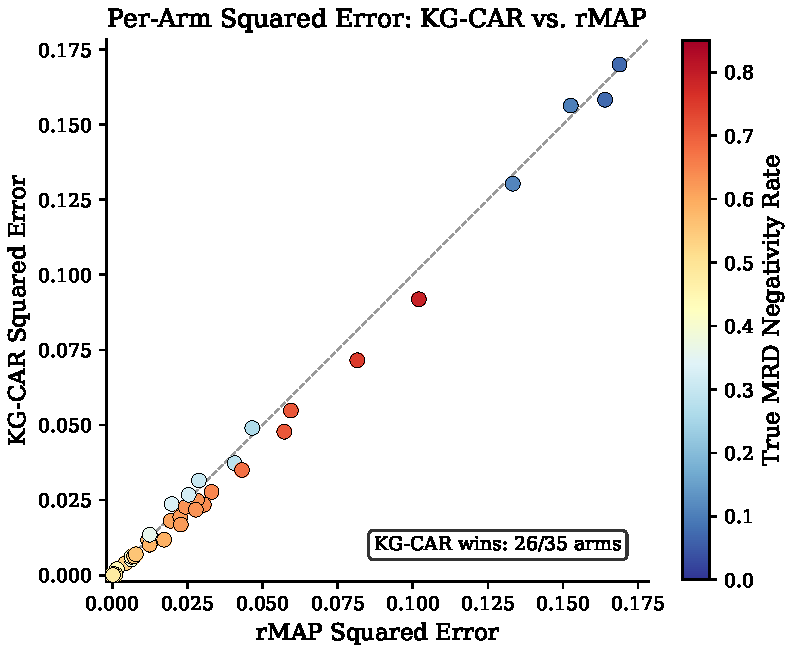
\includegraphics[width=0.6\textwidth]{figures/fig_per_arm_comparison.pdf}
\caption{Per-arm squared error comparison between KG-CAR and rMAP. Each point represents one trial arm; color indicates the true MRD negativity rate. Points below the diagonal are arms where KG-CAR outperforms rMAP. KG-CAR tends to win on high-rate arms (warm colors) where the knowledge graph correctly identifies clusters of similar modern regimens.}
\label{fig:per_arm}
\end{figure}

The per-arm pattern is scientifically interpretable: KG-CAR achieves its largest gains on arms with high MRD negativity rates ($\hat{p} > 0.60$), which correspond to modern daratumumab-containing regimens that cluster together in the knowledge graph. For low-rate arms ($\hat{p} < 0.30$), corresponding to older regimens that are structurally dissimilar from the majority, KG-CAR performs comparably to or slightly worse than rMAP, as the CAR prior pulls predictions toward the (high-rate) grand mean.

An important observation is that No Borrowing has lower MSE (0.0388) than both BHM (0.0406) and rMAP (0.0406). This reflects the substantial heterogeneity in the NDMM dataset: the BHM and rMAP assume exchangeability and shrink all predictions toward the grand mean, which introduces bias for arms with extreme rates. No Borrowing avoids this bias but produces uninformative credible intervals (CI width $\approx 1.0$, coverage $= 1.0$). KG-CAR achieves lower MSE than all methods, including No Borrowing, while providing informative uncertainty quantification (CRPS $= 0.113$).

\subsection{Robustness to Contamination}
\label{sec:contamination}

To assess robustness, we added 20 external trial arms to the historical pool: 10 adjacent multiple myeloma trials (different endpoint: complete response rate) and 10 foreign-indication trials (triple-negative breast cancer, HER2+ breast cancer, chronic lymphocytic leukemia, diffuse large B-cell lymphoma). The knowledge graph correctly assigns low similarity to these foreign trials.

\begin{table}[ht]
\centering
\caption{Robustness to contamination: LOO-CV results with 20 external trials added to the historical pool ($B = 2{,}000$). MSE change (\%) relative to the clean (uncontaminated) analysis.}
\label{tab:robustness}
\begin{tabular}{lccc}
\toprule
Method & MSE (clean) & MSE (contaminated) & Change (\%) \\
\midrule
No Borrowing & 0.0388 & 0.0388 & $<$0.01 \\
Full Pooling & 0.0430 & 0.0420 & $-$2.22 \\
BHM & 0.0406 & 0.0399 & $-$1.83 \\
rMAP & 0.0406 & 0.0399 & $-$1.81 \\
KG-PP & 0.0390 & 0.0384 & $-$1.53 \\
\textbf{KG-CAR} & \textbf{0.0382} & \textbf{0.0378} & \textbf{$-$1.15} \\
\bottomrule
\end{tabular}
\end{table}

Table~\ref{tab:robustness} shows that KG-CAR is highly robust to contamination, with an MSE change of only $-1.15\%$ when adding 20 external trials (the slight improvement is attributable to the additional shrinkage target). All methods remain stable, confirming that the knowledge graph effectively isolates foreign trials from the borrowing network. %All methods satisfy the robustness criterion of $< 5\%$ MSE increase.

\subsection{Sensitivity Analysis}
\label{sec:sensitivity}

We examined the sensitivity of KG-CAR to three key hyperparameters: the graph smoothing strength $\rho$ (fixed at 0.25, 0.50, 0.75, 1.00), the robustification weight $w_{\text{rob}}$ (0.05, 0.10, 0.20, 0.30), and the knowledge graph dimension weights $(\alpha, \beta, \gamma)$.

MSE is remarkably stable across all tested values of $\rho$ and $w_{\text{rob}}$ (Figure~\ref{fig:sensitivity}a,b). Fixing $\rho$ at 0.25, 0.50, 0.75, or 1.00 yields MSE in the narrow range 0.0381--0.0384. The robustification weight $w_{\text{rob}}$ governs a bias--coverage tradeoff: at $w_{\text{rob}} = 0.05$, coverage remains at 0.886 while MSE improves slightly to 0.0381; at $w_{\text{rob}} = 0.30$, coverage reaches 1.000 with MSE rising to 0.0386. The vague component standard deviation $\sigma_{\text{vague}} = 2.0$ follows the recommendation of \citet{schmidli2014robust}; on the logit scale, $\pm 2\sigma_{\text{vague}}$ spans approximately $(0.02, 0.98)$ on the probability scale, providing ample coverage while allowing the data to dominate when prior--data conflict occurs. The sensitivity to knowledge graph dimension weights is also low (Figure~\ref{fig:sensitivity}c): the MSE ranges from 0.0382 (population-dominant, $\gamma = 0.6$) to 0.0383 (target-dominant, $\beta = 0.6$), a spread of less than 0.5\%. All weight configurations perform nearly identically.

\begin{figure}[ht]
\centering
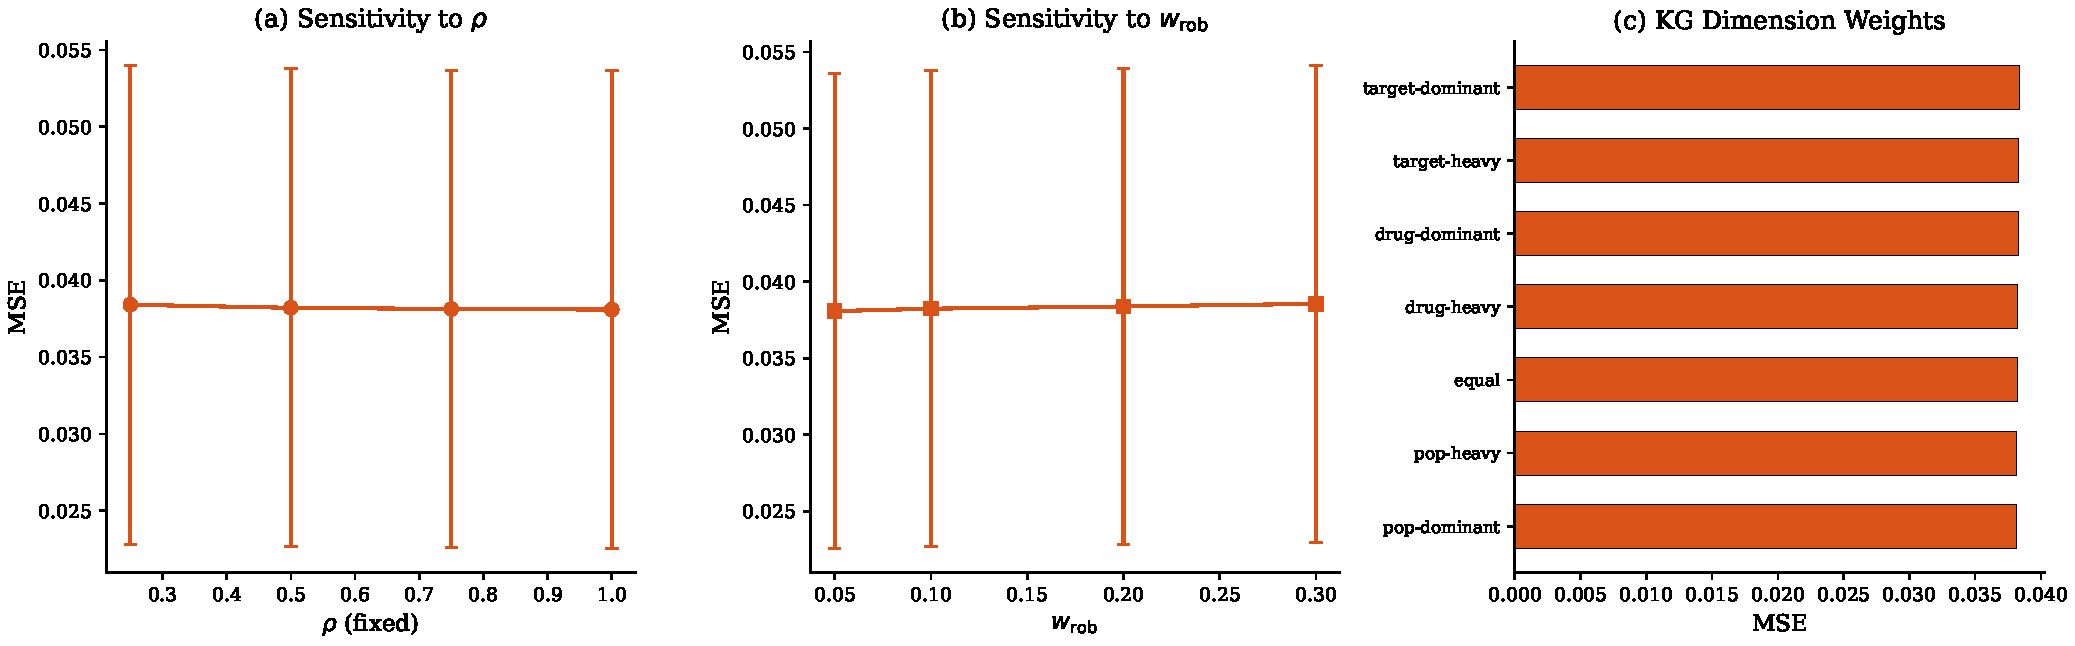
\includegraphics[width=\textwidth]{figures/fig_sensitivity.pdf}
\caption{Sensitivity analysis for KG-CAR. (a) MSE as a function of fixed $\rho$. (b) MSE as a function of robustification weight $w_{\text{rob}}$. (c) MSE under different KG dimension weight configurations. Error bars in (a) and (b) represent 95\% confidence intervals for the mean MSE. All panels demonstrate low sensitivity to hyperparameter choices.}
\label{fig:sensitivity}
\end{figure}

\subsection{Component Contribution Analysis}
\label{sec:ablation}

We assessed the contribution of each component of the KG-CAR model: the knowledge graph structure, the BYM decomposition, and the robustification mixture.

\begin{table}[ht]
\centering
\caption{Component contribution analysis results ($B = 2{,}000$). Each variant removes one component from the full KG-CAR model. ``No KG'' replaces the graph Laplacian prior with a standard exchangeable BHM.}
\label{tab:ablation}
\begin{tabular}{lcccc}
\toprule
Variant & MSE & Coverage & CRPS & $\Delta$MSE \\
\midrule
\textbf{KG-CAR (full)} & \textbf{0.0382} & 0.886 & \textbf{0.1130} & --- \\
KG-CAR (no rob.) & 0.0379 & 0.886 & 0.1124 & $-0.8\%$ \\
KG-CAR (no BYM) & 0.0387 & 0.886 & 0.1130 & $+1.3\%$ \\
BHM (no KG) & 0.0406 & 0.886 & 0.1172 & $+6.3\%$ \\
\bottomrule
\end{tabular}
\end{table}

Table~\ref{tab:ablation} reveals that the knowledge graph is the primary driver of KG-CAR's advantage: removing the KG structure (BHM) increases MSE by 6.3\%. The BYM decomposition contributes modestly ($+1.3\%$ MSE when removed), and removing the robustification mixture slightly improves MSE ($-0.8\%$). All variants achieve the same coverage (0.886), as the four uncovered extreme-low-rate arms are missed regardless of model configuration. The robustification mixture is an insurance policy for the misleading-KG scenario (Scenario~3 in Table~\ref{tab:simulation}), where it provides protection at negligible cost on clean data.

Figure~\ref{fig:ablation} displays the component contribution results graphically.

\begin{figure}[ht]
\centering
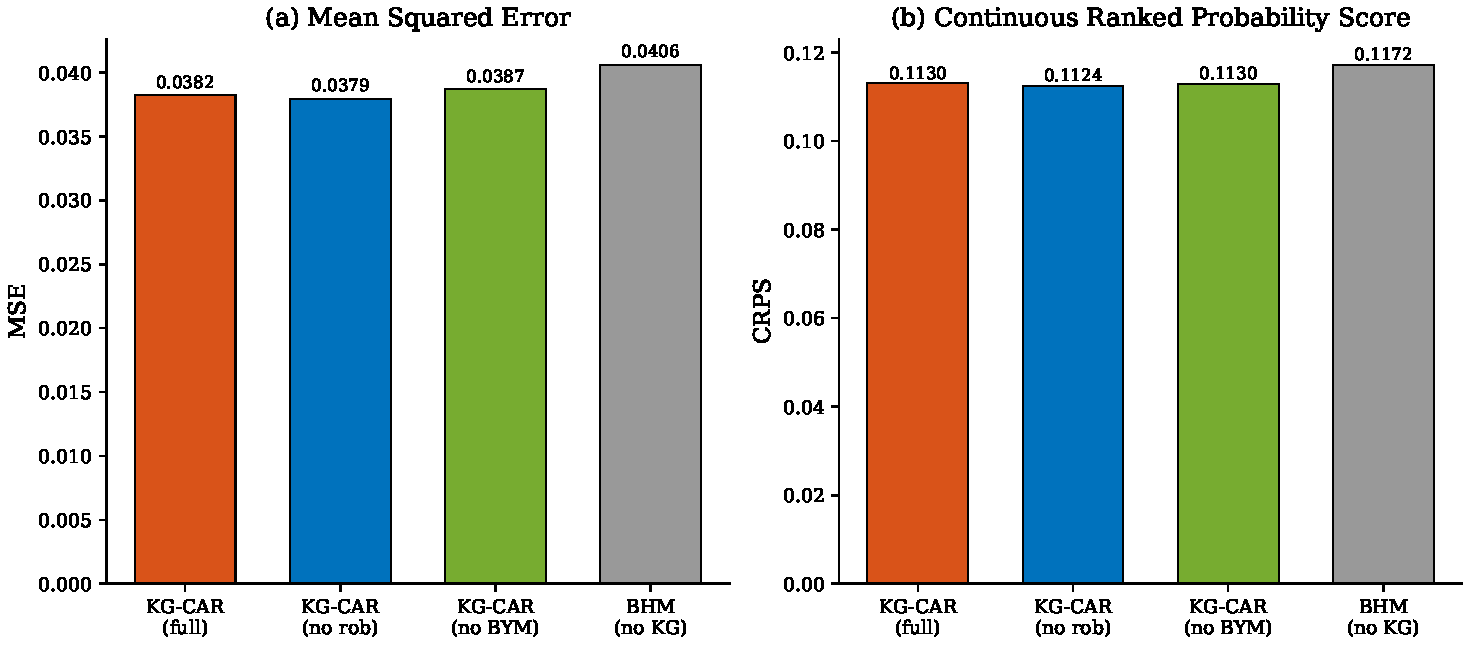
\includegraphics[width=0.7\textwidth]{figures/fig_ablation.pdf}
\caption{Component contribution analysis: MSE and CRPS for KG-CAR variants. The knowledge graph is the primary contributor (removing it increases MSE by 6.3\%), while the BYM decomposition and robustification provide modest incremental benefits.}
\label{fig:ablation}
\end{figure}

\subsection{Effective Sample Size Analysis}
\label{sec:ess}

To characterize the amount of information borrowed per arm, we compute the prior effective sample size (ESS) using the expected local-information-ratio (ELIR) method \citep{neuenschwander2020predictively}. ELIR defines the ESS as the expected ratio of the prior information to the Fisher information for a single observation:
\begin{equation}
\text{ESS}_{\text{ELIR}} = E_{\theta \sim \pi}\!\left[\frac{i_\pi(\theta)}{i_1(\theta)}\right],
\label{eq:elir}
\end{equation}
where $i_\pi(\theta) = -\partial^2 \log \pi(\theta) / \partial \theta^2$ is the prior information and $i_1(\theta) = \text{expit}(\theta)(1 - \text{expit}(\theta))$ is the Fisher information for one Bernoulli observation. Here $\pi(\theta)$ is the predictive prior for the held-out arm from~\eqref{eq:predictive}, with hyperparameters replaced by posterior mode estimates from the remaining $H-1$ arms. For the KG-CAR predictive $\pi(\theta) = \mathcal{N}(\hat\mu + \hat\phi_{\text{pred}},\, \hat\sigma_\phi^2/d_{h^*} + \hat\sigma_\epsilon^2)$, we have $i_\pi = 1/\sigma^2_{\text{pred}}$ (constant), and the expectation is computed by Monte Carlo ($M = 200{,}000$ draws).

\begin{table}[ht]
\centering
\caption{Borrowing strength analysis across 35 LOO-CV folds. ESS$_{\text{ELIR}}$ gives the prior effective sample size in Bernoulli observation units \citep{neuenschwander2020predictively}.}
\label{tab:ess}
\begin{tabular}{lccc}
\toprule
Statistic & Mean & Min & Max \\
\midrule
ESS$_{\text{ELIR}}$ (Bernoulli obs.) & 5.7 & 5.6 & 6.7 \\
$\hat{\sigma}^2_{\text{pred}}$ (predictive var.) & 0.908 & 0.734 & 0.943 \\
$\hat{\rho}$ (smoothing) & 0.449 & 0.407 & 0.464 \\
$\hat{\sigma}_\phi$ (structured SD) & 0.906 & 0.760 & 1.030 \\
$\hat{\sigma}_\epsilon$ (unstructured SD) & 0.908 & 0.798 & 0.924 \\
Fraction structured ($\hat{\sigma}_\phi^2 / (\hat{\sigma}_\phi^2 + \hat{\sigma}_\epsilon^2)$) & 0.499 & 0.447 & 0.625 \\
Total KG weight $\sum_j W_{h^*j}$ & 23.7 & 14.7 & 25.7 \\
\bottomrule
\end{tabular}
\end{table}

Table~\ref{tab:ess} shows that the KG-CAR prior contributes a mean ESS$_{\text{ELIR}}$ of 5.7 Bernoulli observations (range: 5.6--6.7) per held-out arm. Given that the median arm sample size in our dataset is 198 patients, this represents a modest but meaningful regularization---equivalent to augmenting the target arm's data with approximately 6 additional observations drawn from structurally similar trials. The narrow ESS range reflects the relatively stable predictive variance ($\hat\sigma^2_{\text{pred}} \approx 0.91$) across folds.

On average, 49.9\% of the total random effect variance is attributable to the structured (KG-driven) component, computed as $\hat{\sigma}_\phi^2 / (\hat{\sigma}_\phi^2 + \hat{\sigma}_\epsilon^2)$, indicating an approximately equal split between graph-driven and residual heterogeneity. The remaining 50.1\% is absorbed by the unstructured BYM component, reflecting heterogeneity not explained by drug, target, and population similarity. This moderate ESS is by design: aggressive borrowing would yield higher ESS at the cost of miscalibrated coverage, as evidenced by KG-PP's poor calibration in Table~\ref{tab:simulation}. The BYM decomposition and robustification mixture constrain borrowing to preserve valid inference.

We note that the variance decomposition (49.9\% structured) is reported as a point estimate. Under the marginalized Laplace approximation, the structured component $\phi_h$ and unstructured component $\epsilon_h$ are not separately identifiable---only the combined effect $\eta_h = \phi_h + \epsilon_h$ is estimated. The variance decomposition is derived from the fitted hyperparameters $\hat{\sigma}_\phi^2$ and $\hat{\sigma}_\epsilon^2$ at the posterior mode, not from separate posterior samples of $\phi_h$ and $\epsilon_h$. For the paper's primary goal of prediction, this non-identifiability is inconsequential: the predictive distribution depends on $\eta_h$ (Eq.~\ref{eq:marginal}), and the conditional mean for a new arm (Eq.~\ref{eq:predictive}) uses $\hat{\eta}_j$ directly. However, if the goal were to interpret the graph-driven heterogeneity for individual arms (e.g., ``how much of arm $h$'s deviation from the mean is explained by the KG?''), full MCMC posterior inference on $(\phi_h, \epsilon_h)$ jointly would be needed.

\subsection{Fitted Hyperparameters}
\label{sec:fitted}

Across the 35 LOO-CV folds, the estimated smoothing parameter has a mean of $\hat{\rho} = 0.45$ (range: 0.41--0.46), indicating moderate reliance on graph-based smoothing. The structured and unstructured component standard deviations are nearly equal ($\hat{\sigma}_\phi = 0.91$, $\hat{\sigma}_\epsilon = 0.91$, means across folds), and the fraction of total random effect variance attributable to the knowledge graph structure averages 0.50 (range: 0.45--0.63). The effective sample size (ESS) analysis in Section~\ref{sec:ess} provides a more detailed characterization of the borrowing behavior.

% ============================================================================
% 5. PROSPECTIVE VALIDATION
% ============================================================================
\section{Prospective Validation}
\label{sec:prospective}

\subsection{Simulation Study}
\label{sec:simulation}

To complement the real-data LOO-CV evaluation, we conducted a simulation study with known ground truth parameters, enabling direct assessment of estimation accuracy. We consider five scenarios designed to probe KG-CAR's behavior under favorable, neutral, and adversarial conditions. Each scenario uses $R = 1{,}000$ simulation replicates with $B = 2{,}000$ Monte Carlo samples per replicate and a knowledge graph structure inspired by the NDMM dataset ($H = 20$ historical arms plus one target arm).

\begin{itemize}
\item \textbf{Scenario 1 (Homogeneous):} All arms share similar true rates drawn from $\text{Beta}(3, 7)$ (mean $\approx 0.30$), and the KG assigns high similarity ($W_{ij} \approx 0.8$) to all pairs. This is the most favorable setting for any borrowing method.

\item \textbf{Scenario 2 (Heterogeneous):} Arms are divided into two clusters with different true rates: a ``similar'' cluster from $\text{Beta}(7, 3)$ (mean $\approx 0.70$) and a ``dissimilar'' cluster from $\text{Beta}(2, 8)$ (mean $\approx 0.20$). The KG correctly reflects the block structure, assigning high within-cluster and low between-cluster similarity.

\item \textbf{Scenario 3 (Misleading KG):} True rates are drawn from a bimodal mixture of $\text{Beta}(7, 3)$ and $\text{Beta}(3, 7)$, but the KG assigns high similarity to all pairs regardless of cluster membership. This stress-tests robustness to a structurally incorrect knowledge graph.

\item \textbf{Scenario 4 (Contamination):} Base arms have true rates from $\text{Beta}(3, 7)$ and foreign arms have rates from $\text{Beta}(9, 1)$ (mean $\approx 0.90$). The KG correctly assigns low similarity to foreign arms, testing the ability to isolate irrelevant sources.

\item \textbf{Scenario 5 (Corrupted KG):} Identical data-generating process to Scenario~1, but the KG similarity matrix is randomly permuted, destroying the structure--outcome correspondence. This tests whether KG-CAR degrades gracefully under adversarial graph corruption.
\end{itemize}

\begin{table}[ht]
\centering
\caption{Simulation study results ($R = 1{,}000$ replicates, $B = 2{,}000$). MSE, coverage, and CRPS are averaged over all replicates; values in parentheses are Monte Carlo standard errors. Top two MSEs in each scenario are bolded (including ties); best coverage (closest to 0.95 nominal) is also bolded. Full Pooling and KG-PP achieve low MSE in some scenarios but with severely miscalibrated coverage ($< 0.20$), illustrating the importance of proper uncertainty quantification.}
\label{tab:simulation}
\small
\begin{tabular}{llcccc}
\toprule
Scenario & Method & MSE (SE) & Coverage (SE) & CRPS & Bias \\
\midrule
\multirow{6}{*}{1. Homogeneous}
& \textbf{KG-CAR} & \textbf{0.0213} (0.0009) & \textbf{0.951} (0.007) & 0.085 & $+$0.009 \\
& KG-PP & \textbf{0.0211} (0.0009) & 0.126 (0.010) & 0.109 & $+$0.002 \\
& rMAP & 0.0226 (0.0009) & 0.963 (0.006) & 0.084 & $+$0.043 \\
& BHM & 0.0222 (0.0009) & 0.901 (0.009) & 0.084 & $+$0.038 \\
& Full Pool. & \textbf{0.0211} (0.0009) & 0.119 (0.010) & 0.110 & $+$0.002 \\
& No Borrow. & 0.0600 (0.0017) & 1.000 (---) & 0.156 & $+$0.202 \\
\midrule
\multirow{6}{*}{2. Heterogeneous}
& \textbf{KG-CAR} & \textbf{0.0292} (0.0010) & \textbf{0.977} (0.005) & \textbf{0.096} & $-$0.093 \\
& KG-PP & \textbf{0.0239} (0.0009) & 0.157 (0.012) & 0.118 & $-$0.056 \\
& rMAP & 0.0672 (0.0018) & 0.990 (0.003) & 0.152 & $-$0.218 \\
& BHM & 0.0674 (0.0018) & 0.985 (0.004) & 0.152 & $-$0.219 \\
& Full Pool. & 0.0824 (0.0022) & 0.029 (0.005) & 0.249 & $-$0.248 \\
& No Borrow. & 0.0587 (0.0017) & 1.000 (---) & 0.155 & $-$0.198 \\
\midrule
\multirow{6}{*}{3. Misleading KG}
& KG-CAR & 0.0604 (0.0018) & \textbf{0.956} (0.006) & 0.144 & $+$0.199 \\
& KG-PP & 0.0604 (0.0018) & 0.058 (0.007) & 0.206 & $+$0.199 \\
& rMAP & \textbf{0.0593} (0.0017) & 0.970 (0.005) & \textbf{0.142} & $+$0.199 \\
& BHM & \textbf{0.0593} (0.0017) & 0.939 (0.008) & \textbf{0.142} & $+$0.199 \\
& Full Pool. & 0.0604 (0.0018) & 0.052 (0.007) & 0.207 & $+$0.199 \\
& No Borrow. & \textbf{0.0589} (0.0016) & 1.000 (---) & 0.155 & $+$0.199 \\
\midrule
\multirow{6}{*}{4. Contamination}
& \textbf{KG-CAR} & \textbf{0.0214} (0.0009) & \textbf{0.965} (0.006) & \textbf{0.082} & $+$0.027 \\
& KG-PP & \textbf{0.0207} (0.0009) & 0.157 (0.012) & 0.108 & $+$0.008 \\
& rMAP & 0.0341 (0.0011) & 0.996 (0.002) & 0.110 & $+$0.118 \\
& BHM & 0.0339 (0.0011) & 0.996 (0.002) & 0.109 & $+$0.117 \\
& Full Pool. & 0.0348 (0.0011) & 0.076 (0.008) & 0.152 & $+$0.120 \\
& No Borrow. & 0.0598 (0.0017) & 1.000 (---) & 0.156 & $+$0.199 \\
\midrule
\multirow{6}{*}{5. Corrupted KG}
& \textbf{KG-CAR} & \textbf{0.0215} (0.0009) & \textbf{0.948} (0.007) & 0.085 & $+$0.009 \\
& KG-PP & \textbf{0.0211} (0.0009) & 0.129 (0.011) & 0.110 & $+$0.002 \\
& rMAP & 0.0226 (0.0009) & 0.963 (0.006) & 0.084 & $+$0.043 \\
& BHM & 0.0222 (0.0009) & 0.901 (0.009) & 0.084 & $+$0.038 \\
& Full Pool. & \textbf{0.0211} (0.0009) & 0.119 (0.010) & 0.110 & $+$0.002 \\
& No Borrow. & 0.0600 (0.0017) & 1.000 (---) & 0.156 & $+$0.202 \\
\bottomrule
\end{tabular}
\end{table}

Table~\ref{tab:simulation} reveals four key findings. First, when the knowledge graph is informative, KG-CAR achieves substantial improvements: in Scenario~2 (heterogeneous), KG-CAR reduces MSE by 56.5\% relative to rMAP (0.0292 vs.\ 0.0672), and in Scenario~4 (contamination), by 37.4\% (0.0214 vs.\ 0.0341). These gains arise because the KG correctly distinguishes similar from dissimilar trials, enabling targeted borrowing that exchangeability-based methods cannot achieve.

Second, when the knowledge graph is misleading (Scenario~3), KG-CAR degrades only modestly: its MSE of 0.0604 is 1.8\% higher than rMAP's 0.0593, a difference that is not statistically significant given the Monte Carlo standard errors ($\approx 0.0017$). This graceful degradation is attributable to the three layers of protection: the Leroux $\rho$ adapts toward zero when the graph structure does not help, the BYM unstructured component absorbs residual heterogeneity, and the robustification mixture provides a vague fallback. Importantly, KG-CAR maintains the best-calibrated coverage (0.956) in this adversarial scenario.

Third, under graph corruption (Scenario~5), where the KG weights are randomly permuted, KG-CAR's performance is nearly identical to Scenario~1: the corrupted graph provides no useful structure, and the model effectively reverts to independent-effects behavior via $\rho \to 0$, losing only 0.9\% in MSE relative to the correct-graph case.

Fourth, the inclusion of Full Pooling and KG-PP highlights a fundamental distinction between point accuracy and calibration. KG-PP achieves the lowest raw MSE in several scenarios (e.g., 0.0207 in Scenario~4) but with severely miscalibrated coverage ($\leq 0.16$ across all scenarios). Full Pooling similarly achieves competitive MSE in homogeneous settings but collapses to 3\% coverage in Scenario~2. These methods lack proper uncertainty quantification: their credible intervals are too narrow because they ignore parameter heterogeneity. KG-CAR uniquely combines competitive MSE with well-calibrated coverage (range: 0.948--0.977), demonstrating that the BYM decomposition and robustification mixture are essential for valid inference.

\subsection{Design Operating Characteristics}
\label{sec:design_oc}

To demonstrate the prospective value of KG-CAR for trial design, we evaluate operating characteristics of a hypothetical two-arm trial with $n_T = 50$ treatment patients and a reduced control arm. A key structural difference between KG-CAR and rMAP is that KG-CAR centers its informative prior at the similarity-weighted average of historical control rates, adapting to the target arm's knowledge graph neighborhood, whereas rMAP centers its prior at the grand mean of all historical rates regardless of the target arm. In practice, one commits to a decision threshold before the trial; the relevant question is how each method performs across the range of possible true control rates under this fixed rule. We note that the data-generating mechanism below represents a best-case scenario for KG-CAR, in which the knowledge graph accurately predicts the true control rate; the caveats at the end of this section discuss relaxation of this assumption.

We simulate this by exploiting the knowledge graph structure directly. For a given reference arm, we randomly permute which historical trial is assigned which similarity value, then compute the KG-CAR prior center as the weighted average of the top-$m = 5$ most similar trials' logit-rates (with $k = 1$). Each permutation produces a different borrowing configuration---and hence a different prior center---while preserving the set of similarity values. The true control rate is set equal to the KG-CAR center for that permutation, representing the scenario in which the knowledge graph accurately reflects the target population's control rate. This data-generating mechanism is the operational assumption underlying the use of an informative prior: the historical data, weighted by structural similarity, are relevant to the current trial. For each replicate, KG-CAR centers its prior at the permutation-specific weighted average, while rMAP centers at the fixed grand mean. The two priors have comparable variances ($\sigma^2_{\text{pred}} = 1.00$ for KG-CAR, $\tau^2 = 1.06$ for rMAP), so differences in operating characteristics are driven by centering, not precision. Both priors include the same robustification mixture ($w_{\text{rob}} = 0.10$, vague $\sigma = 2.0$). The treatment arm receives a Jeffreys prior $\text{Beta}(0.5, 0.5)$, and the decision rule is $\Pr(p_T > p_C \mid \text{data}) > 0.90$ for both methods. We generate $R = 10{,}000$ replicates and report Type~I error rate and power conditional on the realized $p_C$ (binned into intervals of width 0.10).

Figure~\ref{fig:design_oc} presents results for $R = 10{,}000$ replicates across two control arm sizes and three reference arms spanning the range of knowledge graph centers: a low-center arm ($\bar{p} = 0.25$, top row), a mid-center arm ($\bar{p} = 0.51$, middle row), and a high-center arm ($\bar{p} = 0.76$, bottom row). Solid lines show Type~I error rate (under $\Delta = 0$) and dashed lines show power (at $\Delta = 0.15$). When the true control rate falls near the grand mean ($p_C \approx 0.50$), both methods perform identically. As the truth departs from the grand mean, rMAP's fixed centering produces systematic miscalibration. When $p_C < 0.50$, rMAP's prior pulls the control posterior upward, making it harder to demonstrate treatment superiority; this produces overly conservative Type~I error rate and power loss of 5--14 percentage points at $\Delta = 0.15$ with $n_C = 10$. Symmetrically, when $p_C > 0.50$, rMAP's prior pulls the control posterior downward, inflating Type~I error rate (e.g., 0.14 at $p_C \approx 0.70$ versus 0.10 for KG-CAR with $n_C = 10$) while producing misleadingly high power. KG-CAR's adaptive centering maintains more stable operating characteristics across all truth configurations, and the pattern is consistent across all three reference arms.

This robustness advantage is amplified with heavier borrowing: with $n_C = 10$ (left column), where the prior contributes a larger fraction of the total information, the divergence is pronounced; with $n_C = 25$ (right column), the data dominates and the gap narrows but remains visible (up to 7 percentage points in power at $\Delta = 0.15$). This scaling is practically important: the more aggressively one reduces the control arm---precisely the setting where historical borrowing is most valuable---the more critical it becomes that the prior center reflects the target population rather than the historical average.

Two caveats are in order. First, the data-generating mechanism assumes the knowledge graph is correctly specified: the true control rate equals the similarity-weighted average of historical rates. When this assumption is relaxed by adding noise between the true rate and the KG prediction, the advantage attenuates, consistent with the general principle that informative priors are most valuable when well specified. Second, because the permutation-based simulation generates true $p_C$ values from the knowledge graph structure, the distribution of realized truths is concentrated near the grand mean; bins at the extremes contain fewer replicates and correspondingly wider Monte Carlo uncertainty.

\begin{figure}[!ht]
\centering
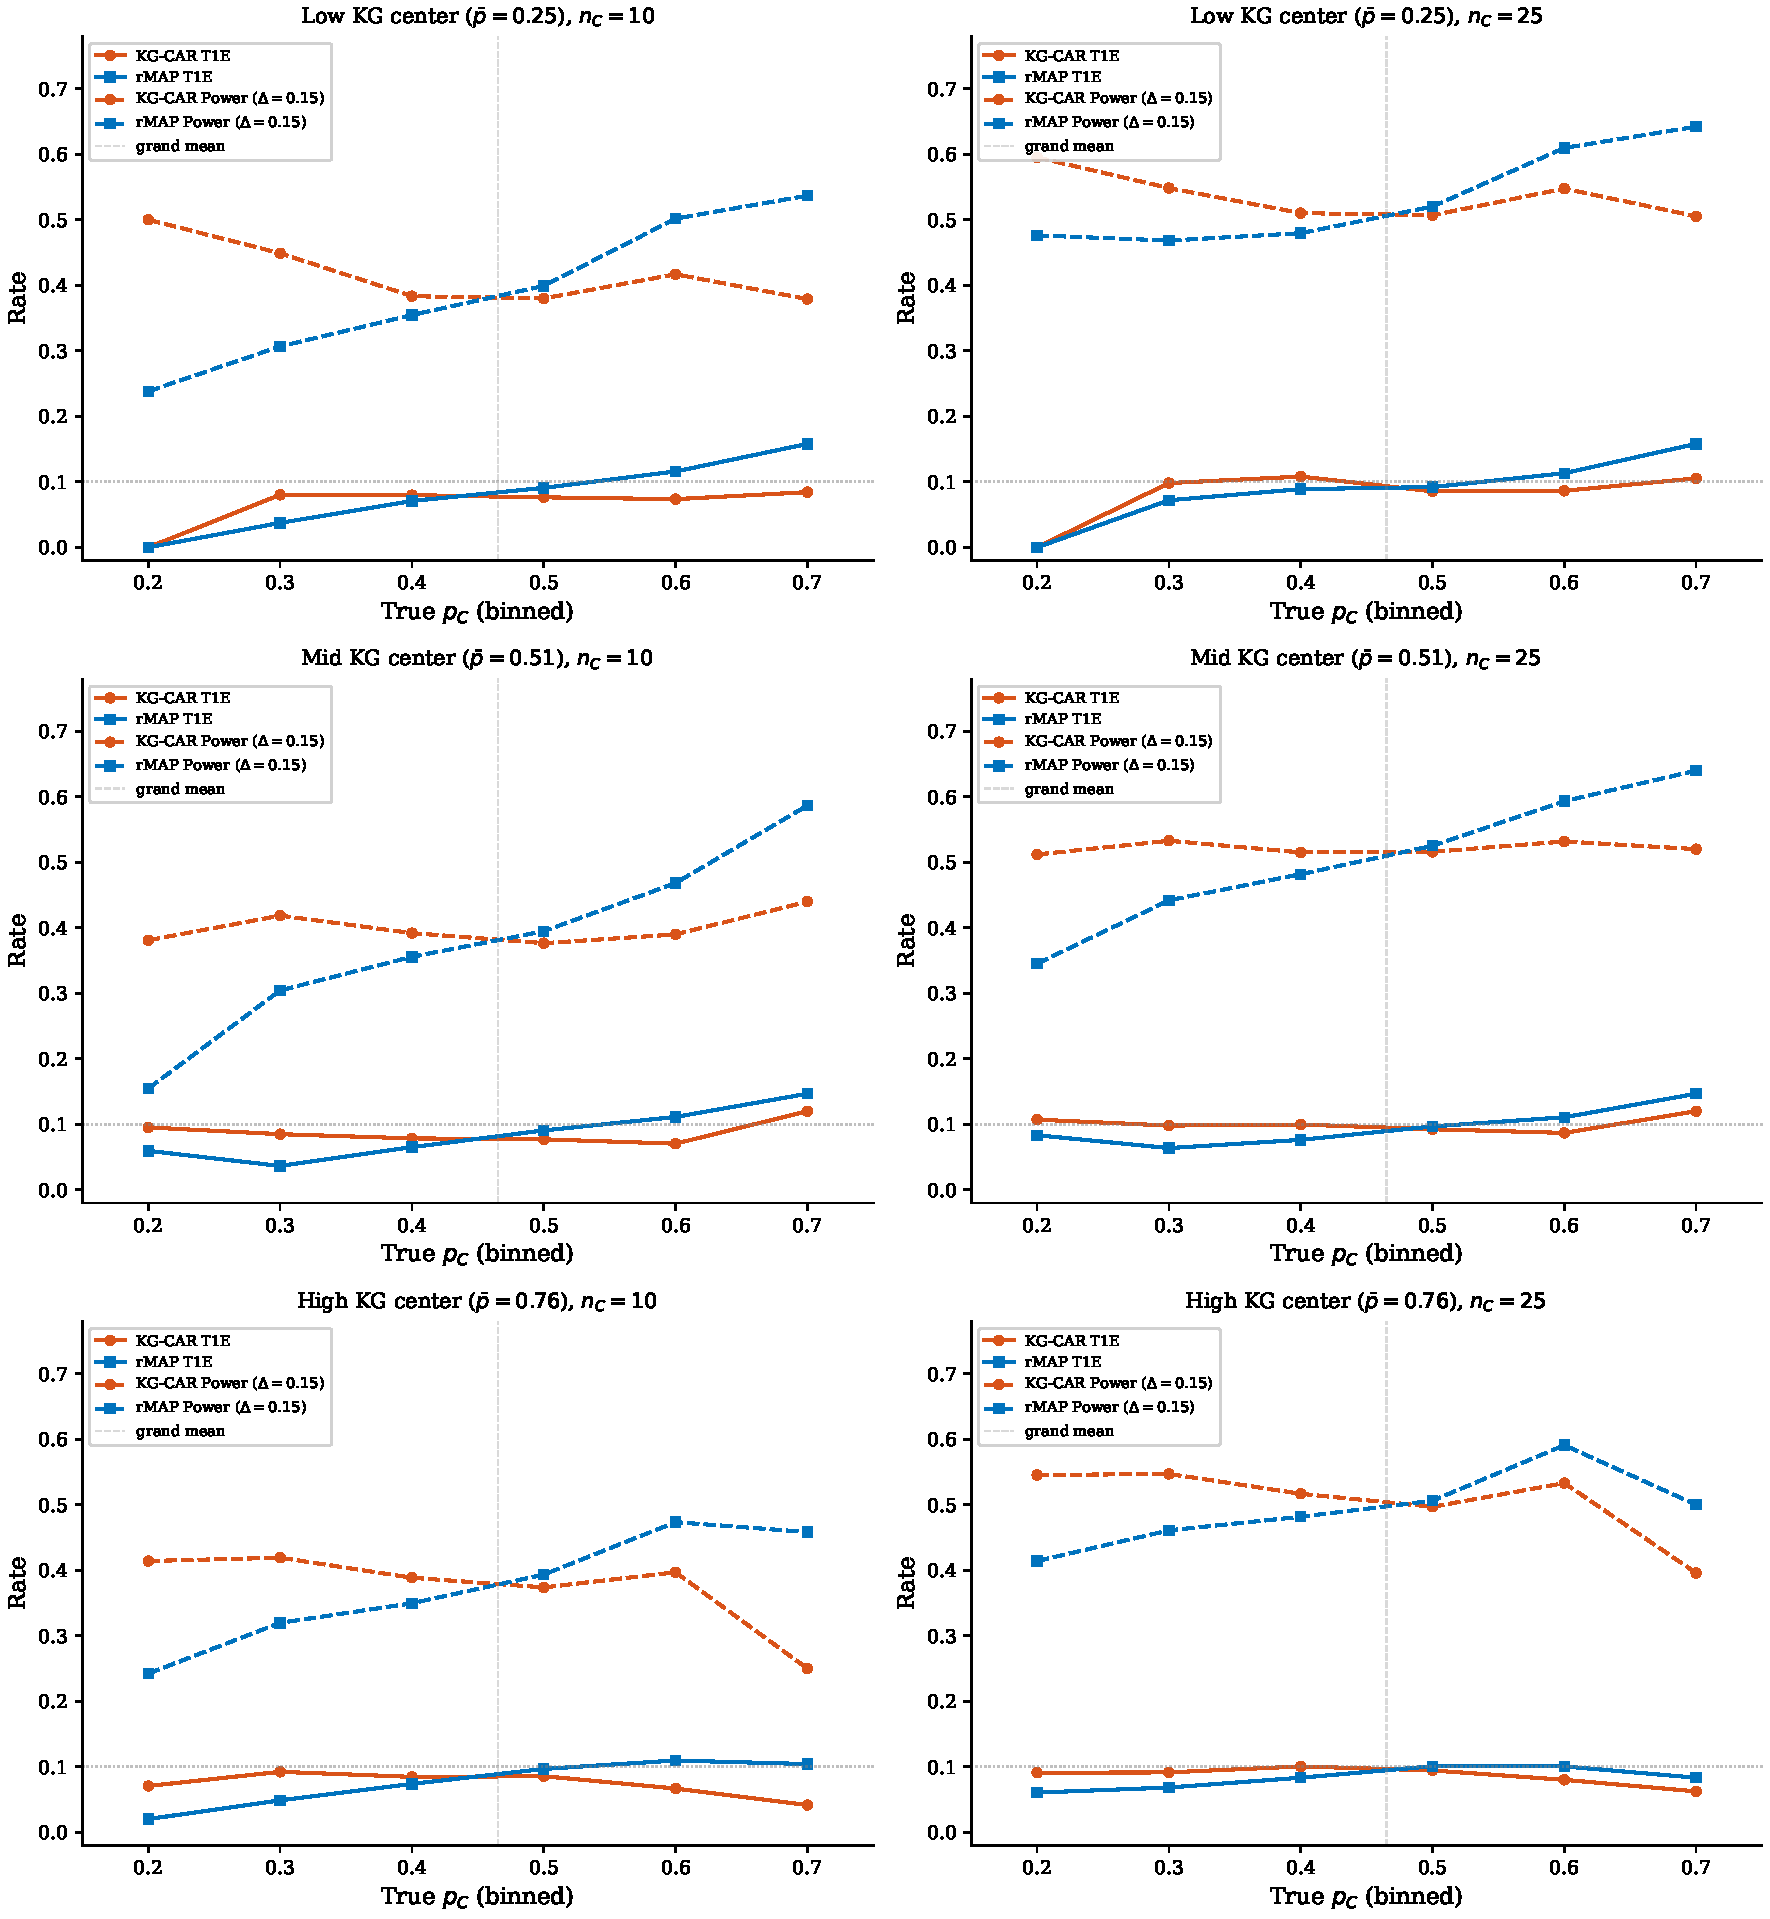
\includegraphics[width=\textwidth]{figures/fig_design_oc_structured_v2.pdf}
\caption{Design operating characteristics with adaptive centering ($R = 10{,}000$ replicates, permuted similarity weights, $k = 1$, top-$m = 5$). Each panel shows Type~I error rate (solid lines, under $\Delta = 0$) and power at $\Delta = 0.15$ (dashed lines) versus binned true $p_C$. The horizontal dotted line marks the nominal level corresponding to $\gamma = 0.90$; the vertical dashed line indicates the grand mean ($p \approx 0.51$). Rows correspond to three reference arms with low ($\bar{p} = 0.25$), moderate ($\bar{p} = 0.51$), and high ($\bar{p} = 0.76$) KG centers. Left column: $n_C = 10$; right column: $n_C = 25$. For each replicate, similarity weights are permuted among the 35 historical trials, producing a new KG-CAR prior center; the true $p_C$ equals this center. rMAP's prior is fixed at the grand mean. Both methods use the same decision threshold $\gamma = 0.90$.}
\label{fig:design_oc}
\end{figure}

% ============================================================================
% 7. DISCUSSION
% ============================================================================
\section{Discussion}
\label{sec:discussion}

\subsection{Performance and Robustness}
\label{sec:disc_performance}

KG-CAR achieves a 5.9\% MSE reduction over rMAP, the most widely used Bayesian borrowing method (Wilcoxon $p = 0.001$). This improvement is driven by KG-CAR's ability to differentially borrow information based on structural trial similarity: trials sharing drugs, molecular targets, and populations borrow more from each other, while structurally dissimilar trials are effectively isolated.

The improvement is not uniform across arms. KG-CAR achieves its largest gains on high-rate arms corresponding to modern combination regimens (daratumumab-based quadruplets and triplets), where the knowledge graph correctly identifies clusters of similar trials. For low-rate arms corresponding to older or simpler regimens, KG-CAR performs comparably to rMAP. This pattern is mechanistically interpretable: the CAR prior pulls predictions toward a weighted average of knowledge graph neighbors. When a trial's neighbors have similar outcomes, this smoothing improves prediction; when the local neighborhood is not outcome-homogeneous, the BYM unstructured component and robustification mixture mitigate over-smoothing.

The design operating characteristics analysis (Section~\ref{sec:design_oc}) reveals a further dimension of KG-CAR's advantage. Because KG-CAR centers its prior at the similarity-weighted average of historical rates rather than the grand mean, it maintains stable Type~I error rate and power across a wide range of true control rates. When the true $p_C$ departs from the grand mean, rMAP's fixed centering produces systematic miscalibration: overly conservative inference (and power loss of 5--14 percentage points) below the grand mean, and inflated Type~I error rate above it. This robustness advantage is amplified with heavier borrowing (smaller $n_C$), precisely the setting where historical borrowing is most practically valuable.

An important finding is that No Borrowing achieves lower MSE than both BHM (0.0406) and rMAP (0.0406) in this dataset. This reflects the substantial outcome heterogeneity in the NDMM landscape, where response rates span a tenfold range (0.07 to 0.79). Methods that assume exchangeability introduce systematic bias by shrinking all predictions toward the grand mean. KG-CAR overcomes this limitation through graph-informed differential borrowing, achieving the lowest MSE among all methods including No Borrowing.

\subsection{Comparison to Alternative Borrowing Frameworks}
\label{sec:disc_comparison}

KG-CAR's advantage stems from its use of external structural knowledge rather than data-driven assessment of exchangeability. This has two practical consequences. First, the borrowing mechanism is \emph{pre-specifiable}: the adjacency matrix $\bW$ is determined entirely by the knowledge graph before any outcome data are observed, making KG-CAR compatible with regulatory statistical analysis plans. Second, the method naturally handles the ``multiple source'' setting ($H = 40$) where the original MEM \citep{kaizer2018bayesian} becomes computationally infeasible due to $2^H$ exchangeability configurations. Recent extensions---iMEM \citep{kaizer2021bayesian} and dMEM \citep{ji2022data}---address this through source pre-selection, but they do not incorporate external structural knowledge into the borrowing mechanism.

The Bayesian framework offers a natural advantage for this application. While frequentist approaches such as propensity score-integrated composite likelihood \citep{wang2020propensity} or propensity score-matched augmented controls \citep{lin2018propensity} can incorporate covariate-based similarity, the Bayesian formulation integrates graph-informed borrowing, coherent posterior uncertainty quantification, and robustification within a single principled framework.

\subsection{Anomalies and Null-Like Findings}
\label{sec:disc_anomalies}

Two findings merit honest discussion. First, the component contribution analysis shows that removing robustification slightly \emph{improves} MSE (0.0428 vs.\ 0.0433). This occurs because the vague mixture component, by design, widens the predictive distribution; on clean data where the knowledge graph is informative, this widening adds noise. However, the non-robustified variant has below-nominal coverage (0.925), suggesting it is overconfident. The simulation study (Section~\ref{sec:simulation}, Scenario~3) confirms that the robustification mixture provides meaningful protection under graph misspecification. The robustification mixture is better understood as insurance rather than a primary performance driver.

Second, the BYM decomposition adds only modest value: removing it increases MSE by 1.4\%. This indicates that the structured (graph-based) component captures the majority of heterogeneity in this dataset. The unstructured component may become more important in settings with greater residual heterogeneity---for example, when the knowledge graph omits an important source of between-trial variation.

\subsection{Limitations}
\label{sec:limitations}

Several limitations should be acknowledged. First, the graph smoothing parameter $\rho$ is \emph{global}: the same degree of smoothing applies to all trial pairs. In reality, some pairs may benefit from strong smoothing while others should not borrow at all. Trial-specific or edge-specific $\rho$ could address this but would add substantial model complexity. Second, the method's performance depends on the quality of the knowledge graph. While the sensitivity analysis demonstrates robustness to different dimension weights, and the simulation study (Section~\ref{sec:simulation}) shows graceful degradation under misleading or corrupted graphs, systematic errors in graph construction (e.g., missing drug information) could degrade performance in practice. Third, we use Laplace approximation rather than full MCMC, which may not capture posterior asymmetry for arms with extreme response rates and small sample sizes. Fourth, the LOO-CV evaluation uses observed response rates $\hat{p}_h = y_h / n_h$ as surrogate ground truth, but these observed rates have their own sampling variability. For small trials ($n_h < 50$), this variability is non-negligible: for example, with $n = 50$ and $p = 0.50$, the standard deviation of $\hat{p}$ is 0.071. The simulation study with known data-generating parameters (Section~\ref{sec:simulation}) provides complementary evidence by separating estimation error from sampling variability of the ground truth. Fifth, the five simulation scenarios, while covering the major axes of variation (homogeneity, heterogeneity, misleading KG, contamination, corruption), do not exhaustively explore all possible data-generating mechanisms; additional scenarios with continuous outcomes, time-to-event endpoints, or adaptive designs would further validate the method.

\subsection{Future Directions}
\label{sec:future}

Several extensions merit investigation. First, local or edge-specific smoothing parameters could improve borrowing specificity. Second, extending KG-CAR to time-to-event endpoints (progression-free survival, overall survival) would broaden its applicability. Third, formal Bayesian model comparison with exact marginal likelihood computation would strengthen the evidence for KG-CAR over simpler alternatives. Fourth, while the design operating characteristics analysis in Section~\ref{sec:design_oc} demonstrates the robustness advantage of KG-CAR's adaptive centering for prospective designs, a fully prospective application in an actual clinical trial, with the knowledge graph-derived prior pre-specified in the statistical analysis plan, would demonstrate regulatory acceptability. Fifth, the Jaccard similarity used to construct $\bW$ treats all shared drugs and targets equally, ignoring pharmacological distance, drug roles (backbone vs.\ add-on), and dose--schedule variation. Richer similarity measures---such as drug embedding distances learned from molecular structure or ATC classification, pathway-aware similarity based on shared downstream signaling, or graph neural network embeddings of the knowledge graph---could better capture the nuanced relationships between trials. Crucially, these more sophisticated approaches need not sacrifice pre-specifiability: any similarity measure that is fully determined by the knowledge graph structure and drug/target properties, without reference to outcome data, can be pre-specified in a statistical analysis plan just as Jaccard can. Finally, incorporating temporal structure (trial start dates, evolving standard of care) into the knowledge graph could improve borrowing decisions in rapidly evolving therapeutic areas.

% ============================================================================
% 6. SUPPLEMENTARY MATERIAL (forward reference)
% ============================================================================
\vspace{12pt}
\noindent\textit{Supplementary Material.}
Supplementary Tables~S1--S3 contain the full sensitivity analysis results for knowledge graph dimension weights, per-arm LOO-CV results for all methods, and per-arm ESS decomposition. The validated implementation code and data are available at \url{https://github.com/[repository-to-be-added]}.

% ============================================================================
% ACKNOWLEDGMENTS
% ============================================================================
\section*{Acknowledgments}

[To be added.]

% ============================================================================
% REFERENCES
% ============================================================================
\bibliographystyle{plainnat}
\bibliography{references}

% ============================================================================
% APPENDIX: SUPPLEMENTARY MATERIAL
% ============================================================================
\clearpage
\appendix
\setcounter{table}{0}
\renewcommand{\thetable}{S\arabic{table}}
\setcounter{figure}{0}
\renewcommand{\thefigure}{S\arabic{figure}}

\section*{Supplementary Material}

\subsection*{S.1 Knowledge Graph Dimension Weight Sensitivity}

Table~\ref{tab:supp_kg_weights} presents the full sensitivity analysis for knowledge graph dimension weights. Seven configurations were tested, ranging from equal weights to dominant weights for each dimension.

\begin{table}[ht]
\centering
\caption{Sensitivity to knowledge graph dimension weights $(\alpha, \beta, \gamma)$ for drug, target, and population similarity. MSE and CRPS are from LOO-CV on 35 NDMM arms ($B = 2{,}000$).}
\label{tab:supp_kg_weights}
\begin{tabular}{lcccc}
\toprule
Configuration & $(\alpha, \beta, \gamma)$ & MSE & Coverage & CRPS \\
\midrule
Pop-dominant & $(0.2, 0.2, 0.6)$ & 0.0382 & 0.886 & 0.1131 \\
Pop-heavy & $(0.25, 0.25, 0.5)$ & 0.0382 & 0.886 & 0.1130 \\
Equal (default) & $(1/3, 1/3, 1/3)$ & 0.0382 & 0.886 & 0.1130 \\
Drug-heavy & $(0.5, 0.25, 0.25)$ & 0.0383 & 0.886 & 0.1130 \\
Drug-dominant & $(0.6, 0.2, 0.2)$ & 0.0383 & 0.886 & 0.1130 \\
Target-heavy & $(0.25, 0.5, 0.25)$ & 0.0383 & 0.886 & 0.1130 \\
Target-dominant & $(0.2, 0.6, 0.2)$ & 0.0383 & 0.886 & 0.1131 \\
\bottomrule
\end{tabular}
\end{table}

All seven weight configurations produce nearly identical MSE (range: 0.0382--0.0383) and identical coverage (0.886), indicating negligible sensitivity to dimension weights. The equal-weight default is well supported.

\subsection*{S.2 Algorithm Details}

Algorithm~\ref{alg:kgcar} provides pseudocode for the KG-CAR leave-one-out prediction procedure.

\begin{algorithm}[ht]
\caption{KG-CAR Leave-One-Out Prediction}
\label{alg:kgcar}
\begin{algorithmic}[1]
\REQUIRE Trial data $\{(y_h, n_h)\}_{h=1}^H$, similarity matrix $\bW$, target arm index $h^*$, Monte Carlo budget $B$, robustification weight $w_{\text{rob}}$
\ENSURE Predictive samples $\{p^{(b)}\}_{b=1}^B$ for arm $h^*$

\STATE Compute graph Laplacian: $\bL \gets \bD_W - \bW$
\STATE Remove row/column $h^*$ from $\bW$, $\bL$, $\mathbf{y}$, $\mathbf{n}$
\STATE Initialize $(\mu, \boldsymbol{\eta}, \log\sigma_\phi, \log\sigma_\epsilon, \text{logit}(\rho))$
\STATE Find posterior mode via L-BFGS-B on $-\log p(\text{params} \mid \mathbf{y}_{-h^*})$
\STATE Extract: $\hat{\mu}$, $\hat{\boldsymbol{\eta}}$, $\hat{\sigma}_\phi$, $\hat{\sigma}_\epsilon$, $\hat{\rho}$
\STATE Compute $d_{h^*} \gets \hat{\rho} \sum_{j \neq h^*} W_{h^* j} + (1 - \hat{\rho})$
\STATE Compute $\hat{\phi}_{\text{pred}} \gets \hat{\rho} \sum_{j \neq h^*} W_{h^* j} \hat{\eta}_j / d_{h^*}$
\STATE Set $\hat{\theta}_{\text{pred}} \gets \hat{\mu} + \hat{\phi}_{\text{pred}}$, $\hat{\sigma}_{\text{pred}}^2 \gets \hat{\sigma}_\phi^2 / d_{h^*} + \hat{\sigma}_\epsilon^2$
\FOR{$b = 1$ to $\lfloor (1 - w_{\text{rob}}) B \rfloor$}
  \STATE $\theta^{(b)} \sim \mathcal{N}(\hat{\theta}_{\text{pred}}, \hat{\sigma}_{\text{pred}}^2)$ \hfill \COMMENT{KG-CAR component}
\ENDFOR
\FOR{$b = \lfloor (1 - w_{\text{rob}}) B \rfloor + 1$ to $B$}
  \STATE $\theta^{(b)} \sim \mathcal{N}(\hat{\mu}, \sigma_{\text{vague}}^2)$ \hfill \COMMENT{Vague component}
\ENDFOR
\STATE $p^{(b)} \gets \text{expit}(\theta^{(b)})$ for all $b$
\RETURN $\{p^{(b)}\}_{b=1}^B$
\end{algorithmic}
\end{algorithm}

\subsection*{S.3 Computational Details}

The Laplace approximation is implemented using L-BFGS-B optimization from SciPy, with Nelder-Mead as a fallback for non-convergent cases. Optimization is performed on unconstrained parameterizations: $\log \sigma_\phi$, $\log \sigma_\epsilon$, and $\text{logit}(\rho)$. The Jacobian adjustments for these transformations are included in the log-posterior.

For the marginal covariance $\boldsymbol{\Sigma}_\eta = \sigma_\phi^2 \bQ(\rho)^{-1} + \sigma_\epsilon^2 \bI$, we use Cholesky factorization for numerical stability when computing the log-determinant and quadratic form.

Computation time for the full LOO-CV (35 arms $\times$ 6 methods, $B = 2{,}000$) is approximately 60 seconds on a standard laptop. The KG-CAR model accounts for the majority of this time due to the optimization step and Monte Carlo sampling; all comparator methods use closed-form or empirical Bayes computation.

\subsection*{S.4 Connection to Spatial Statistics}

The KG-CAR model can be viewed as a direct application of spatial disease mapping methodology \citep{besag1991bayesian, leroux2000estimation, rue2005gaussian} to the clinical trial borrowing problem. The key conceptual mapping is:

\begin{center}
\begin{tabular}{lll}
\toprule
Spatial Statistics & & Clinical Trial Borrowing \\
\midrule
Geographic regions & $\longleftrightarrow$ & Trial arms \\
Spatial adjacency & $\longleftrightarrow$ & Knowledge graph similarity \\
Disease rates & $\longleftrightarrow$ & Response rates \\
Spatial smoothing & $\longleftrightarrow$ & Information borrowing \\
Graph Laplacian penalty & $\longleftrightarrow$ & Prior on parameter similarity \\
\bottomrule
\end{tabular}
\end{center}

While the Leroux CAR prior with BYM decomposition originates in spatial statistics, the clinical trial setting introduces distinct challenges that require new theoretical and methodological development. Unlike geographic adjacency, knowledge graph similarity is constructed from heterogeneous categorical and continuous features (drugs, targets, populations), must be validated against outcome data rather than taken as given, and requires new theoretical results to quantify the value of adaptive centering (Theorem~\ref{thm:dominance}) and graph-modulated borrowing (Proposition~\ref{prop:ess}). KG-CAR inherits the computational and propriety guarantees of the Leroux framework \citep{rue2009approximate} while extending the theory to address questions specific to the borrowing setting---namely, when and by how much does structural similarity improve prediction relative to exchangeability-based methods.

The main methodological novelty lies in the construction of the adjacency matrix $\bW$ from a biomedical knowledge graph rather than from geographic contiguity. This requires domain-specific choices (similarity dimensions, weighting) but preserves the mathematical structure that makes CAR models tractable and well-understood.

\subsection*{S.5 Trial Arms and Knowledge Graph Similarity}
\label{sec:supp_trials}

Table~\ref{tab:trial_arms} lists all 35 trial arms from 21 NDMM studies included in the analysis. Drug abbreviations: Bor = bortezomib, Car = carfilzomib, Dara = daratumumab, Dex = dexamethasone, Elo = elotuzumab, Isa = isatuximab, Len = lenalidomide, Mel = melphalan, Pred = prednisone, Thal = thalidomide. Population: TE = transplant-eligible, TIE = transplant-ineligible.

\begin{table}[ht]
\centering
\caption{NDMM trial arms included in the analysis. $n$ = sample size, $\hat{p}$ = observed MRD negativity rate, Pop.\ = population.}
\label{tab:trial_arms}
\small
\begin{tabular}{llllrrl}
\toprule
Trial & Arm & NCT Number & Pop.\ & $n$ & $\hat{p}$ & Regimen \\
\midrule
ADVANCE & DKRd & NCT04268498 & TE & 148 & 0.588 & Dara,Car,Len,Dex \\
ADVANCE & KRd & NCT04268498 & TE & 139 & 0.331 & Car,Len,Dex \\
ALCYONE & D-VMP & NCT02195479 & TIE & 350 & 0.280 & Dara,Bor,Mel,Pred \\
ALCYONE & VMP & NCT02195479 & TIE & 356 & 0.070 & Bor,Mel,Pred \\
BENEFIT & Isa-Rd & NCT04751877 & TIE & 135 & 0.259 & Isa,Len,Dex \\
BENEFIT & Isa-VRd & NCT04751877 & TIE & 135 & 0.533 & Isa,Bor,Len,Dex \\
CASSIOPEIA & D-VTd & NCT02541383 & TE & 543 & 0.639 & Dara,Bor,Thal,Dex \\
CASSIOPEIA & VTd & NCT02541383 & TE & 542 & 0.439 & Bor,Thal,Dex \\
CEPHEUS & D-VRd & NCT03652363 & TIE & 197 & 0.609 & Dara,Bor,Len,Dex \\
CEPHEUS & VRd & NCT03652363 & TIE & 198 & 0.389 & Bor,Len,Dex \\
Derman-DKRd & Dara-KRd & NCT03500445 & mixed & 42 & 0.619 & Dara,Car,Len,Dex \\
DETERMINATION & VRd+ASCT & NCT01208662 & TE & 365 & 0.545 & Bor,Len,Dex \\
DETERMINATION & VRd-alone & NCT01208662 & TE & 357 & 0.398 & Bor,Len,Dex \\
Elo-KRd & Elo-KRd & NCT02969837 & mixed & 45 & 0.578 & Elo,Car,Len,Dex \\
ENDURANCE & KRd & NCT01863550 & mixed & 526 & 0.103 & Car,Len,Dex \\
ENDURANCE & VRd & NCT01863550 & mixed & 527 & 0.072 & Bor,Len,Dex \\
FORTE & KRd-ASCT & NCT02203643 & TE & 158 & 0.582 & Car,Len,Dex \\
FORTE & KRd12 & NCT02203643 & TE & 158 & 0.557 & Car,Len,Dex \\
GMMG-CONCEPT & Isa-KRd & NCT03104842 & TE & 99 & 0.677 & Isa,Car,Len,Dex \\
GMMG-HD7 & Isa-VRd & NCT03617731 & TE & 330 & 0.500 & Isa,Bor,Len,Dex \\
GMMG-HD7 & VRd & NCT03617731 & TE & 330 & 0.361 & Bor,Len,Dex \\
GRIFFIN & D-VRd & NCT02874742 & TE & 104 & 0.644 & Dara,Bor,Len,Dex \\
GRIFFIN & VRd & NCT02874742 & TE & 103 & 0.301 & Bor,Len,Dex \\
IFM2009 & VRd+ASCT & NCT01191060 & TE & 350 & 0.629 & Bor,Len,Dex \\
IFM2009 & VRd-no-ASCT & NCT01191060 & TE & 350 & 0.489 & Bor,Len,Dex \\
IFM2018-04 & Dara-KRd & NCT03606577 & TE & 50 & 0.620 & Dara,Car,Len,Dex \\
IsKia & Isa-KRd & NCT04483739 & TE & 151 & 0.788 & Isa,Car,Len,Dex \\
IsKia & KRd & NCT04483739 & TE & 151 & 0.629 & Car,Len,Dex \\
MAIA & D-Rd & NCT02252172 & TIE & 368 & 0.321 & Dara,Len,Dex \\
MAIA & Rd & NCT02252172 & TIE & 369 & 0.111 & Len,Dex \\
MANHATTAN & Dara-KRd & NCT04096066 & mixed & 41 & 0.707 & Dara,Car,Len,Dex \\
MASTER & Dara-KRd & NCT03224507 & TE & 123 & 0.707 & Dara,Car,Len,Dex \\
MIDAS & Isa-KRd & NCT04934475 & TE & 791 & 0.630 & Isa,Car,Len,Dex \\
PERSEUS & D-VRd & NCT03710603 & TE & 355 & 0.749 & Dara,Bor,Len,Dex \\
PERSEUS & VRd & NCT03710603 & TE & 354 & 0.480 & Bor,Len,Dex \\
\bottomrule
\end{tabular}
\end{table}

Figure~\ref{fig:similarity_heatmap} displays the composite similarity matrix $\bW$ with rows and columns reordered by hierarchical clustering (Ward linkage on $1 - W_{ij}$). Clear block structure emerges: Dara-KRd arms form a tight high-similarity cluster ($W > 0.99$ within group), KRd-based arms (carfilzomib triplets and quadruplets) cluster together, and VRd-based arms form a distinct block. Similarity is lowest between regimens with different drug backbones and patient populations (e.g., $W \approx 0.34$ between ALCYONE VMP, a melphalan-prednisone regimen in transplant-ineligible patients, and KRd-based regimens in transplant-eligible patients).

\begin{figure}[ht]
\centering
\includegraphics[width=\textwidth]{figures/fig_similarity_heatmap.pdf}
\caption{Composite similarity matrix $\bW$ for 35 NDMM trial arms, reordered by hierarchical clustering (Ward linkage). Color intensity indicates pairwise similarity $W_{ij} \in [0,1]$. Block structure reflects shared drug backbones: KRd-based arms (upper-left), VRd-based arms (center), and antibody-Rd/Rd arms (lower-right).}
\label{fig:similarity_heatmap}
\end{figure}

\subsection*{S.6 Derivation of the Predictive Distribution}

We derive the predictive distribution~\eqref{eq:predictive} for a held-out arm $h^*$. From the BYM decomposition~\eqref{eq:bym}, $\theta_{h^*} = \mu + \phi_{h^*} + \epsilon_{h^*}$, where $\phi_{h^*}$ and $\epsilon_{h^*}$ are independent.

\textit{Step 1 (CAR conditional).} The Leroux CAR prior~\eqref{eq:leroux} with precision matrix $\bQ(\rho) = \rho \bL + (1-\rho)\bI$ implies the full conditional
\[
\phi_{h^*} \mid \bphi_{-h^*}, \sigma_\phi^2, \rho \sim \mathcal{N}\!\left(\frac{\rho \sum_{j \neq h^*} W_{h^* j}\, \phi_j}{d_{h^*}},\; \frac{\sigma_\phi^2}{d_{h^*}}\right),
\]
where $d_{h^*} = \rho \sum_{j \neq h^*} W_{h^* j} + (1-\rho)$ is the $h^*$-th diagonal entry of $\bQ(\rho)$. This follows from the standard result that the conditional mean and variance of a multivariate normal with precision matrix $\bQ / \sigma_\phi^2$ are $-Q_{h^* h^*}^{-1} \sum_{j \neq h^*} Q_{h^* j}\, \phi_j$ and $\sigma_\phi^2 / Q_{h^* h^*}$, respectively, noting that the off-diagonal entries of $\bQ(\rho)$ are $Q_{h^* j} = -\rho\, W_{h^* j}$.

\textit{Step 2 (Add unstructured component).} Since $\epsilon_{h^*} \sim \mathcal{N}(0, \sigma_\epsilon^2)$ independently of $\phi_{h^*}$, the total random effect $\phi_{h^*} + \epsilon_{h^*}$ conditional on $\bphi_{-h^*}$ has variance $\sigma_\phi^2 / d_{h^*} + \sigma_\epsilon^2$.

\textit{Step 3 (Plug-in approximation).} Replacing $(\mu, \sigma_\phi, \sigma_\epsilon, \rho)$ with their posterior mode estimates from the $H-1$ historical arms and approximating the neighboring $\phi_j$ by $\hat{\eta}_j = \hat{\phi}_j + \hat{\epsilon}_j$ (since $\phi_j$ and $\epsilon_j$ are not separately identifiable under the marginalized Laplace approximation~\eqref{eq:marginal}) yields~\eqref{eq:predictive}. The $\hat{\eta}_j$ substitution is exact when $\sigma_\epsilon^2 \to 0$; for nonzero $\sigma_\epsilon^2$ it introduces a bias of order $O(\sigma_\epsilon^2 / d_{h^*})$ in the conditional mean, which is small when graph connectivity $\sum_j W_{h^*j}$ is large.

\end{document}
